\documentclass[UTF8,a4paper,12pt]{ctexart}

\usepackage{geometry}
\usepackage{amsmath}
\usepackage{amssymb}
\usepackage{graphicx}
\usepackage{booktabs}
\usepackage{float}
\usepackage{caption}
\usepackage{hyperref}
\usepackage{enumitem}
\usepackage{array}

\geometry{left=2.5cm,right=2.5cm,top=2.6cm,bottom=2.6cm}
\hypersetup{colorlinks=true,linkcolor=black,citecolor=black,urlcolor=blue}
\setlist{itemsep=0.2em,topsep=0.4em}

\title{基于稀疏动力学识别与物理-机器学习混合修正的 Lorenz 混沌系统预测边界分析}
\author{小组成员：钟兴涛、黄宇轩、郝致祺\\课程名称：人工智能导论}
\date{\today}

\begin{document}

\maketitle

\begin{abstract}
本文以 Lorenz 混沌系统为对象，研究机器学习模型在非线性动力系统中的短期状态转移拟合能力、动力学结构识别能力和预测边界。原始单变量任务只预测 $x(t+10\Delta t)$，容易得到很高精度；本文将其扩展为三维状态转移预测 $\mathbf{s}_t\to\mathbf{s}_{t+k}$，并从预测步长、递归多步预测和不同初始条件三个角度分析误差如何增长。

在此基础上，本文进一步加入 SINDy 稀疏动力学识别和物理-机器学习混合修正实验。SINDy 从轨迹数据中恢复出接近 Lorenz 方程的稀疏结构，例如 $dx/dt\approx -9.994x+9.994y$、$dy/dt\approx27.952x-0.991y-0.999xz$、$dz/dt\approx0.999xy-2.665z$。Hybrid correction 则构造参数有偏的物理模型（$\rho=26$）并用机器学习学习其残差，将一步状态 RMSE 从 0.0786 降低到 0.0003--0.0006，并将 500 步 rollout 的有效预测时间从 0.35 个 Lyapunov time 提升到至少 2.25 个 Lyapunov time。本文的结论不是“机器学习已经解决混沌系统长期预测”，而是：机器学习可以近似短期局部动力学映射，稀疏识别可以揭示方程结构，混合修正可以改善不完美物理模型，但长期逐点预测仍受到混沌系统初值敏感性和误差放大的限制。
\end{abstract}

\noindent\textbf{关键词：} Lorenz 系统；混沌；状态转移预测；残差学习；回声状态网络；预测步长；递归预测；AI4SCI

\section{引言}

科学预测是人工智能与科学计算交叉领域中的重要问题。许多自然系统由确定性方程控制，但非线性耦合和初值敏感性会使其长期行为难以预测。Lorenz 系统最初来源于大气对流模型，是混沌理论中的经典案例 \cite{lorenz1963}。该系统的轨迹在相空间中形成著名的蝴蝶形吸引子，并对初始状态极其敏感。

原始课程任务要求根据 Lorenz 系统当前状态 $(x_t,y_t,z_t)$ 预测 10 个采样步长后的 $x$ 分量。该任务适合展示监督学习回归的基本流程，但单一分量、固定短步长的高精度并不足以反映混沌系统预测中的误差增长、递归推演稳定性和轨迹泛化问题。因此，本文将研究对象从单变量短期预测扩展为完整三维状态转移预测，并重点分析机器学习模型在混沌系统中的预测边界。

本文围绕以下问题展开：

\begin{enumerate}
    \item 机器学习模型能否从数据中学习 Lorenz 系统的完整三维状态转移映射？
    \item 当预测步长（prediction horizon）增大时，预测误差如何变化？
    \item 当一步模型被递归用于多步预测（recursive rollout）时，误差是否会累积？
    \item 在不重新训练的情况下，模型能否泛化到不同初始条件生成的新轨迹？
    \item 残差学习、输出标准化、激活函数和回声状态网络（ESN）是否能改善状态转移建模？
\end{enumerate}

本文的主要贡献包括：

\begin{enumerate}
    \item 将原始单变量短期预测扩展为三维状态转移预测，使任务更接近动力系统建模问题；
    \item 通过预测步长、递归多步预测和初始条件泛化三个实验刻画 Lorenz 系统中的预测边界；
    \item 比较直接 MLP、Residual MLP、输出标准化、激活函数和 ESN 对状态转移学习的影响，突出模型结构改进的作用与局限；
    \item 引入 SINDy 稀疏动力学识别和物理-机器学习混合修正，使项目从单纯预测升级为动力学结构发现与不完美物理模型误差校正。
\end{enumerate}

\subsection{相关工作与研究定位}

Lorenz 系统是研究非线性动力学和混沌现象的经典模型，其确定性方程和初值敏感性使其成为检验预测模型的重要基准 \cite{lorenz1963,strogatz2015}。机器学习方法可以从模拟数据中拟合局部状态转移关系，而 ESN 所属的 reservoir computing 方法则常用于时序动态系统建模 \cite{lukosevicius2009}。本文不追求提出新的动力系统算法，而是以 AI 导论课程项目为定位，比较常见机器学习模型在短期拟合、长期递推和轨迹泛化中的表现差异。

\section{数学背景与问题定义}

\subsection{Lorenz 系统}

Lorenz 系统由以下三个耦合常微分方程组成：

\begin{equation}
\frac{dx}{dt}=\sigma(y-x),
\end{equation}

\begin{equation}
\frac{dy}{dt}=x(\rho-z)-y,
\end{equation}

\begin{equation}
\frac{dz}{dt}=xy-\beta z.
\end{equation}

本文采用经典参数设置：

\begin{equation}
\sigma=10,\quad \rho=28,\quad \beta=\frac{8}{3}.
\end{equation}

在该参数组合下，系统表现出典型混沌行为。混沌系统的关键特点是短期局部演化具有可学习规律，但长期轨迹会因初始误差和模型误差被非线性动力学放大而变得难以精确预测 \cite{strogatz2015}。

\subsection{从单变量预测到状态转移预测}

原始任务定义为：

\begin{equation}
(x_t,y_t,z_t)\rightarrow x_{t+10}.
\end{equation}

增强后的主要任务定义为完整状态转移预测。令系统状态向量为

\begin{equation}
\mathbf{s}_t=(x_t,y_t,z_t),
\end{equation}

则预测步长（horizon）为 $k$ 的监督学习任务为

\begin{equation}
\mathbf{s}_t\rightarrow \mathbf{s}_{t+k}=(x_{t+k},y_{t+k},z_{t+k}).
\end{equation}

其中 $k\in\{1,5,10,20,50,100,200,500\}$。该设定比单一 $x$ 分量预测更接近动力系统状态预测任务，也能直接分析预测步长对误差的影响。

\subsection{递归 rollout}

除直接预测 $\mathbf{s}_{t+k}$ 外，本文还训练一步状态转移模型：

\begin{equation}
\hat{\mathbf{s}}_{t+1}=f_\theta(\mathbf{s}_t).
\end{equation}

在 rollout 阶段，只给定初始真实状态 $\mathbf{s}_t$，之后重复使用模型输出作为下一步输入：

\begin{equation}
\hat{\mathbf{s}}_{t+i+1}=f_\theta(\hat{\mathbf{s}}_{t+i}).
\end{equation}

这一实验用于观察一步预测误差在连续递推中的累积现象。

\section{数据生成与实验设计}

\subsection{数据生成}

本文不使用外部数据集，而是通过 \texttt{scipy.integrate.solve\_ivp} 数值求解 Lorenz 方程 \cite{virtanen2020}。基础训练轨迹初始条件为 $(1,1,1)$，模拟时间范围为 $[0,50]$，采样点数为 10000，采样步长约为

\begin{equation}
\Delta t \approx 0.0050005.
\end{equation}

图 \ref{fig:lorenz} 展示了该参数设置下的三维吸引子结构。

\begin{figure}[H]
\centering
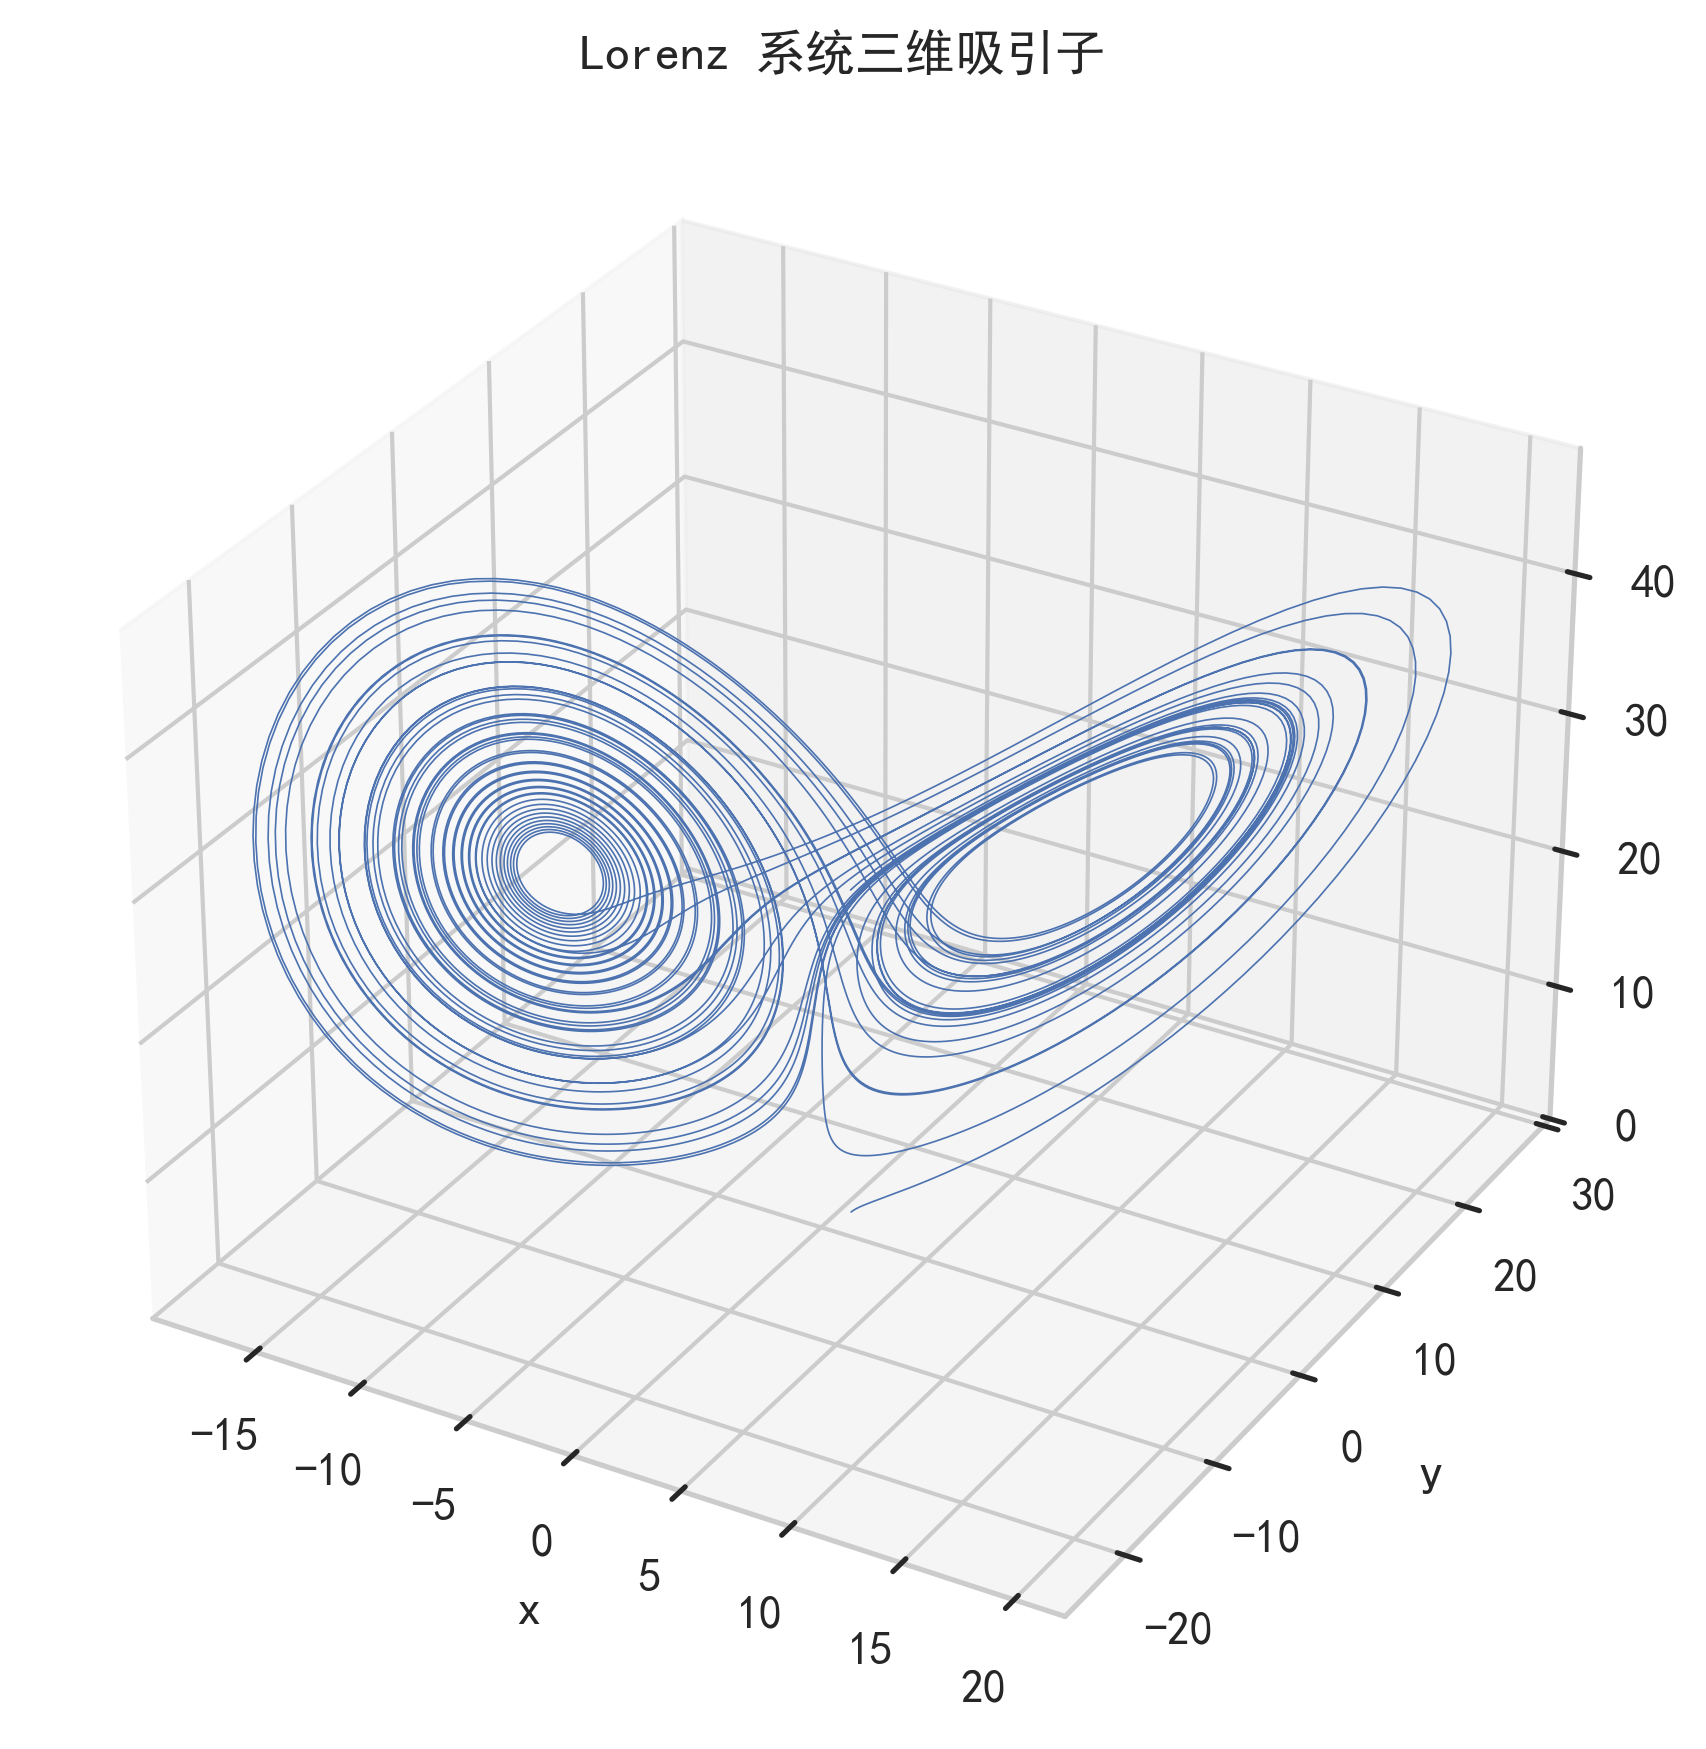
\includegraphics[width=0.78\textwidth]{figures/lorenz_attractor.png}
\caption{Lorenz 系统三维吸引子轨迹图}
\label{fig:lorenz}
\end{figure}

\subsection{模型设置}

本文比较以下模型，并为每类模型设置明确角色：

\begin{enumerate}
    \item \textbf{Persistence Model}：直接将当前状态作为未来状态预测，是最简单的连续性基线。
    \item \textbf{Linear Regression}：用线性映射近似局部状态转移，是局部线性化基线。
    \item \textbf{Random Forest Regressor}：传统非线性机器学习强基线，用于检验非线性树模型在不同预测步长下的稳定性。
    \item \textbf{Direct MLP}：直接预测未来状态 $\mathbf{s}_{t+k}$，作为神经网络状态预测的基本形式。
    \item \textbf{Residual MLP}：预测状态变化量 $\Delta\mathbf{s}=\mathbf{s}_{t+k}-\mathbf{s}_t$，再还原 $\hat{\mathbf{s}}_{t+k}=\mathbf{s}_t+\widehat{\Delta\mathbf{s}}$。该设计更贴近数值积分中的“当前状态加增量”思想，是本文模型增强部分的重点。
    \item \textbf{回声状态网络（ESN）}：使用固定随机 reservoir 和线性 readout 的 reservoir computing 模型，作为动力系统时间序列模型对照。
    \item \textbf{SINDy}：在多项式候选函数库中使用稀疏回归识别控制方程，用于回答模型是否能从数据中恢复动力学结构。
    \item \textbf{Hybrid correction}：构造参数有偏的 Lorenz 物理模型，并训练机器学习残差修正器学习真实一步状态与不完美物理预测之间的偏差。
\end{enumerate}

模型使用 scikit-learn 实现 \cite{pedregosa2011}；ESN 使用轻量 NumPy 实现。对输入特征使用 StandardScaler 标准化，且只在训练集上拟合，再应用到测试集。对 MLP 的输出目标 $Y=(x,y,z)$ 或残差目标 $\Delta Y$ 也使用 StandardScaler，并在评价前反标准化回原始物理尺度，以避免不同状态分量的数值尺度影响训练。

\subsection{SINDy 与混合修正设置}

SINDy 实验使用中心差分估计导数：

\begin{equation}
\dot{\mathbf{s}}_t\approx\frac{\mathbf{s}_{t+1}-\mathbf{s}_{t-1}}{2\Delta t}.
\end{equation}

候选函数库设为

\begin{equation}
\Theta(\mathbf{s})=[1,x,y,z,x^2,xy,xz,y^2,yz,z^2],
\end{equation}

然后使用 sequential thresholded least squares 进行稀疏回归，阈值设为 0.05。该实验的目标不是提升一步 RMSE，而是检查数据驱动方法能否恢复 Lorenz 方程的少量关键项。

Hybrid correction 实验中，真实系统参数仍为 $\rho=28$，不完美物理模型故意设为 $\rho=26$，其余参数保持不变。先用该错误物理模型计算一步预测 $\mathbf{s}^{phys}_{t+1}$，再训练残差模型：

\begin{equation}
\mathbf{r}_{t+1}=\mathbf{s}_{t+1}-\mathbf{s}^{phys}_{t+1},
\end{equation}

最终混合预测为

\begin{equation}
\hat{\mathbf{s}}^{hybrid}_{t+1}=\mathbf{s}^{phys}_{t+1}+\hat{\mathbf{r}}_{t+1}.
\end{equation}

本文比较 imperfect physics、pure ML residual MLP、Hybrid RF 和 Hybrid MLP，并在 500 步递归 rollout 中评估误差累积。

\subsection{评价指标}

对单变量原始任务，继续使用 RMSE、MAE 和 $R^2$。对完整三维状态预测，本文定义状态 RMSE：

\begin{equation}
RMSE_{state}=\sqrt{\frac{1}{n}\sum_{i=1}^{n}\|\mathbf{s}_i-\hat{\mathbf{s}}_i\|_2^2}.
\end{equation}

同时计算 $x,y,z$ 各分量的 RMSE、MAE、$R^2$，并报告三个分量 $R^2$ 的平均值 $R^2_{mean}$。

为了更符合混沌系统评价习惯，本文还引入有效预测时间（valid prediction time）。Lorenz63 最大 Lyapunov 指数近似取 0.9，因此一个 Lyapunov time 约为 $1/0.9\approx1.11$ 个物理时间单位。当 rollout 的状态误差超过训练轨迹状态标准差范数的 0.4 倍时，认为逐点预测失效，并将失效前时间换算为 Lyapunov time。同时报告长期统计量，包括各状态分量的均值、标准差、最小值、最大值和分布对比。

\section{实验结果}

\subsection{原始单变量短期预测结果}

表 \ref{tab:original_metrics} 给出了原始 $x(t+10\Delta t)$ 预测任务结果。非线性模型在该任务上取得很高精度，说明 Lorenz 系统短期局部演化映射可以被机器学习模型拟合。

\begin{table}[H]
\centering
\caption{原始单变量短期预测结果}
\label{tab:original_metrics}
\begin{tabular}{lccc}
\toprule
模型 & RMSE & MAE & $R^2$ \\
\midrule
Persistence Model & 2.1653 & 1.7657 & 0.9208 \\
线性回归 & 0.5679 & 0.4556 & 0.9946 \\
随机森林 & 0.0887 & 0.0504 & 0.9999 \\
MLP & 0.0779 & 0.0574 & 0.9999 \\
\bottomrule
\end{tabular}
\end{table}

因此，该实验在本文中主要作为起点：它说明短期局部映射是可学习的，但不能单独支撑长期混沌预测结论。

\subsection{预测步长敏感性（horizon sensitivity）}

表 \ref{tab:horizon_metrics} 展示了若干代表性预测步长下的三维状态预测结果，完整结果保存在结果目录中。可以看到，$k=10$ 时 Random Forest 和 MLP 均能保持较低状态 RMSE；当 $k$ 增大到 100 和 500 后，误差显著增加，$R^2_{mean}$ 也明显下降。

\begin{table}[H]
\centering
\caption{不同预测步长下的三维状态预测代表性结果}
\label{tab:horizon_metrics}
\begin{tabular}{rlcc}
\toprule
Horizon & 模型 & State RMSE & $R^2_{mean}$ \\
\midrule
10 & Random Forest & 0.2987 & 0.9996 \\
10 & MLP & 0.4572 & 0.9991 \\
100 & Random Forest & 4.3280 & 0.9164 \\
100 & MLP & 2.2369 & 0.9781 \\
500 & Random Forest & 12.7868 & 0.2607 \\
500 & MLP & 13.6858 & 0.1591 \\
\bottomrule
\end{tabular}
\end{table}

图 \ref{fig:horizon_rmse} 更直观地展示了预测步长与状态 RMSE 的关系。随着 $k$ 增大，Persistence 和 Linear Regression 快速失效；非线性模型在中短期内更稳健，但在较长预测步长下也出现明显退化。

\begin{figure}[H]
\centering
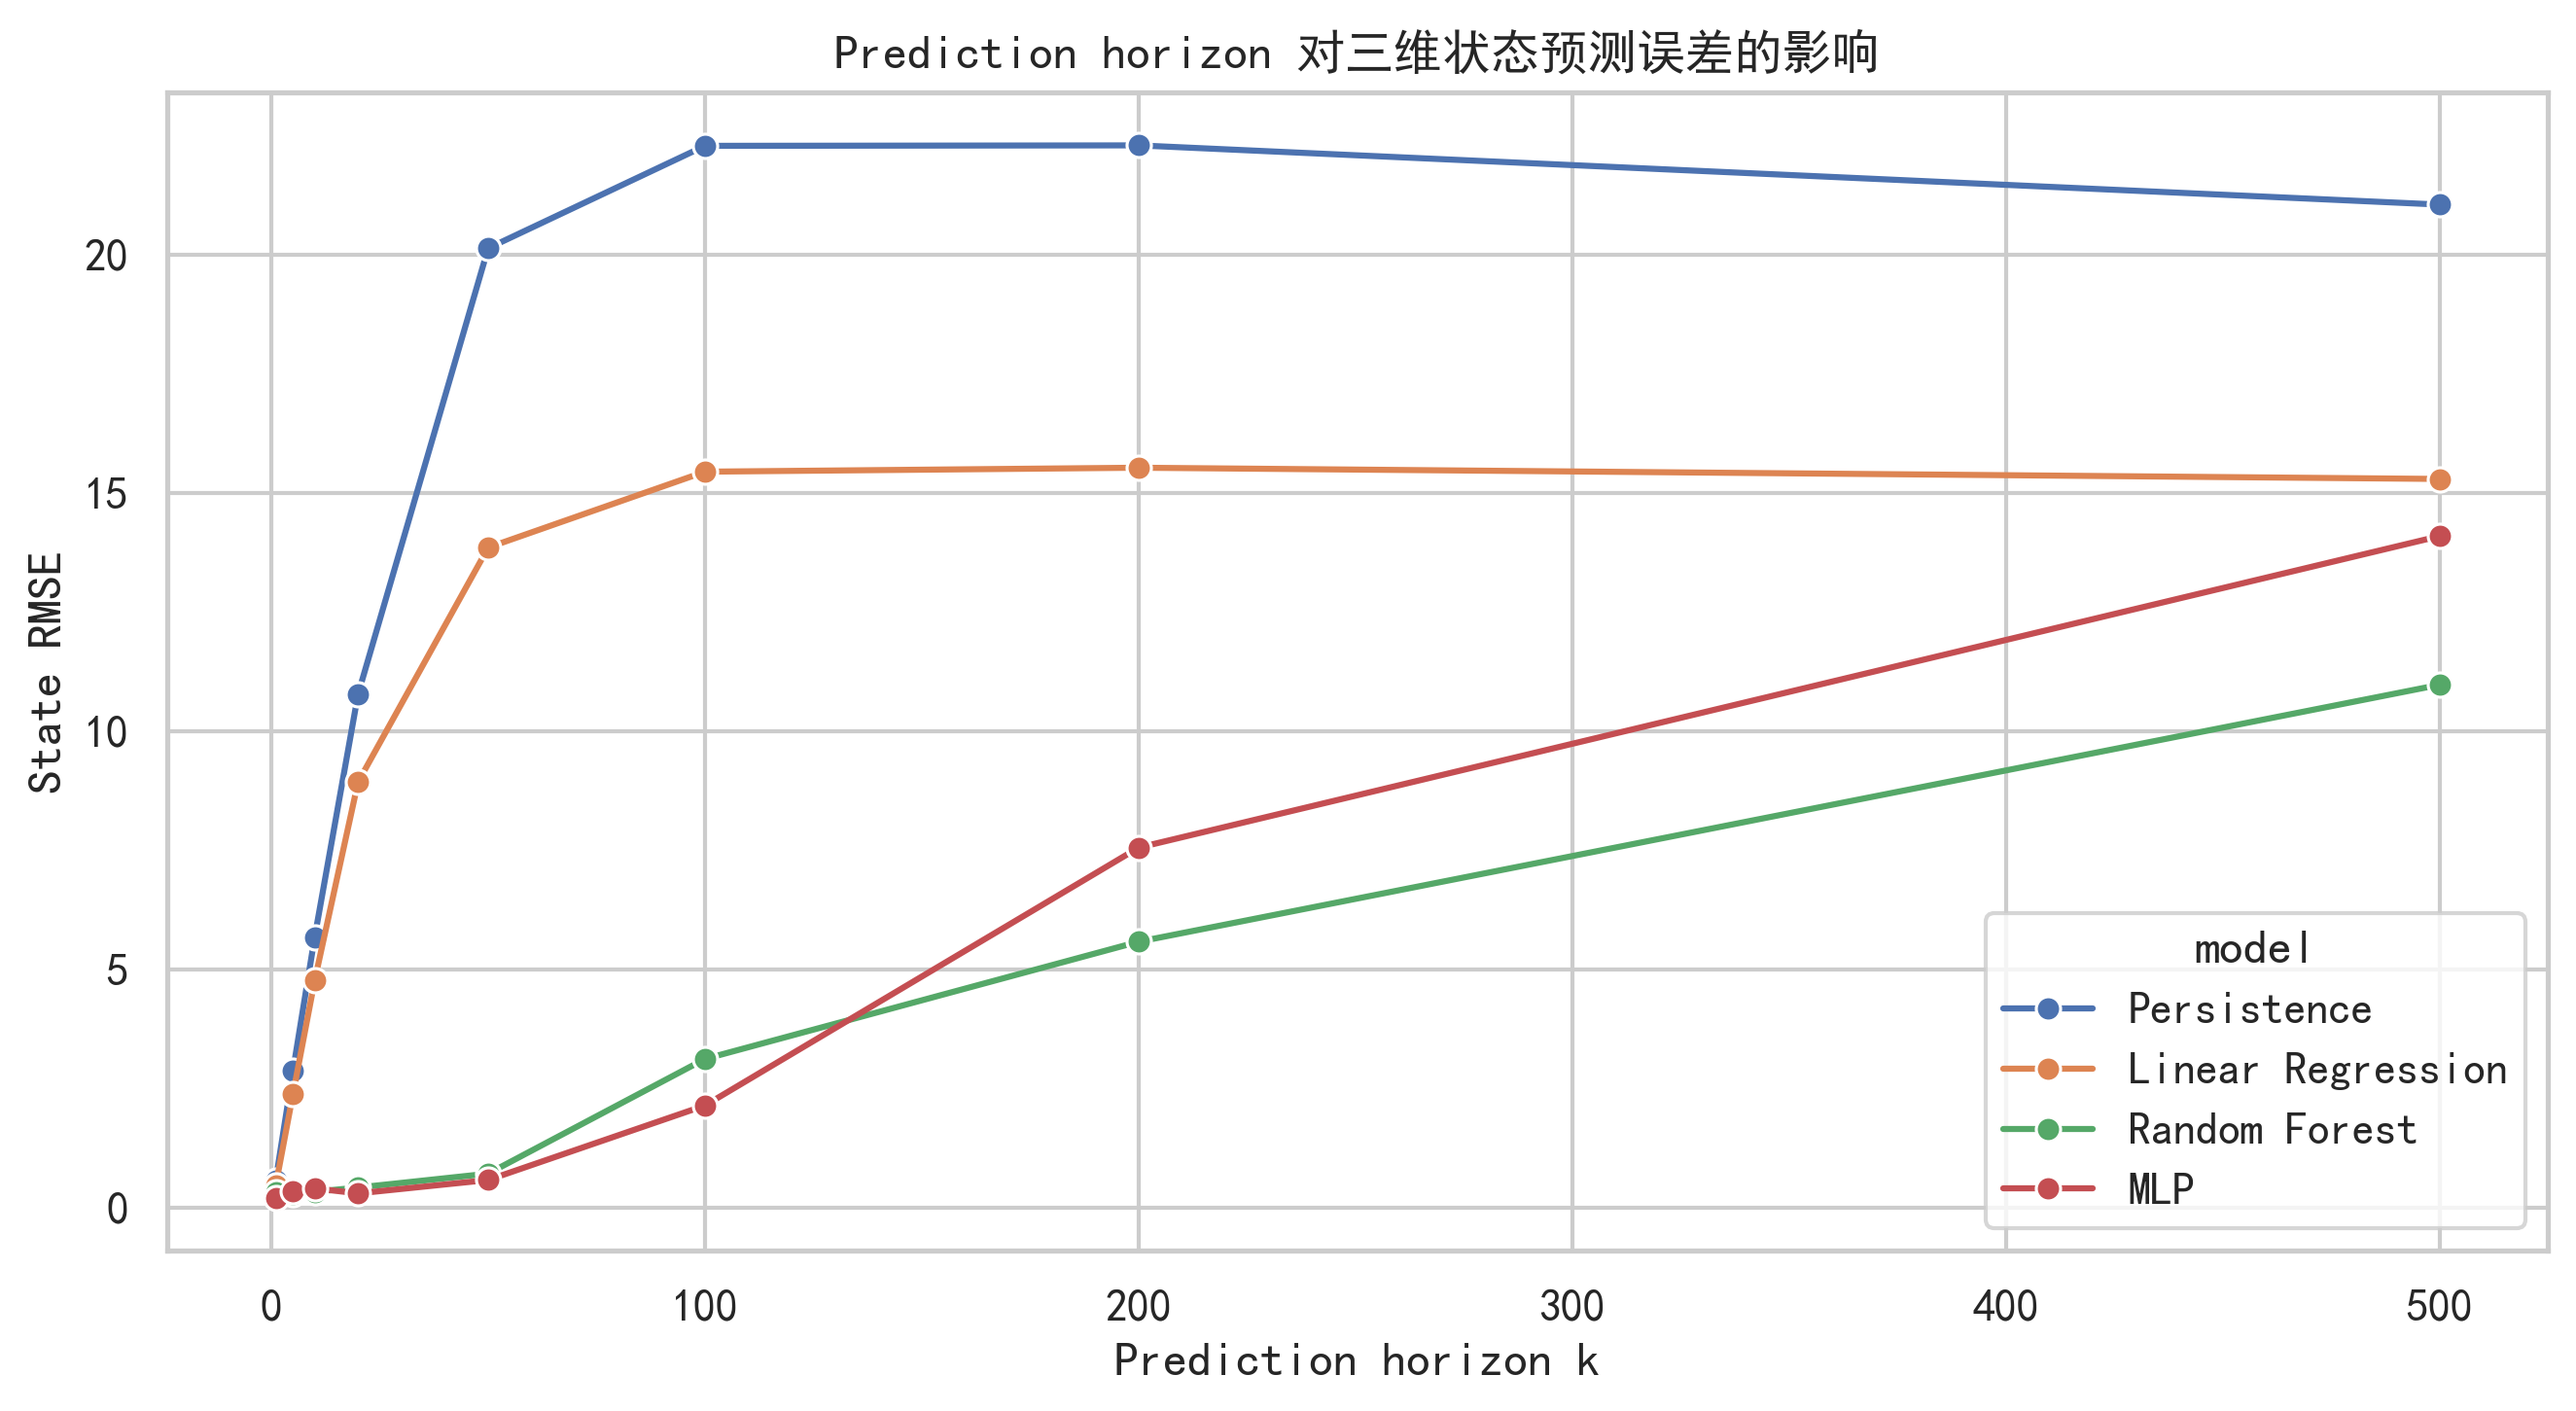
\includegraphics[width=0.86\textwidth]{figures/horizon_vs_rmse.png}
\caption{预测步长对三维状态预测误差的影响。纵轴采用对数尺度，以突出短、中、长预测步长下误差增长的整体趋势。}
\label{fig:horizon_rmse}
\end{figure}

\subsection{递归多步预测（rollout）}

直接预测 $\mathbf{s}_{t+k}$ 时，每个测试样本仍使用真实当前状态作为输入；而长期推演更接近递归多步预测：模型必须不断使用自己的预测结果继续向前推进。图 \ref{fig:rollout_error} 显示了 500 步 rollout 中累计状态 RMSE 的变化。500 步结束时，Linear Regression、Random Forest、MLP 的累计状态 RMSE 分别约为 20.2040、14.3255、18.0711。

\begin{figure}[H]
\centering
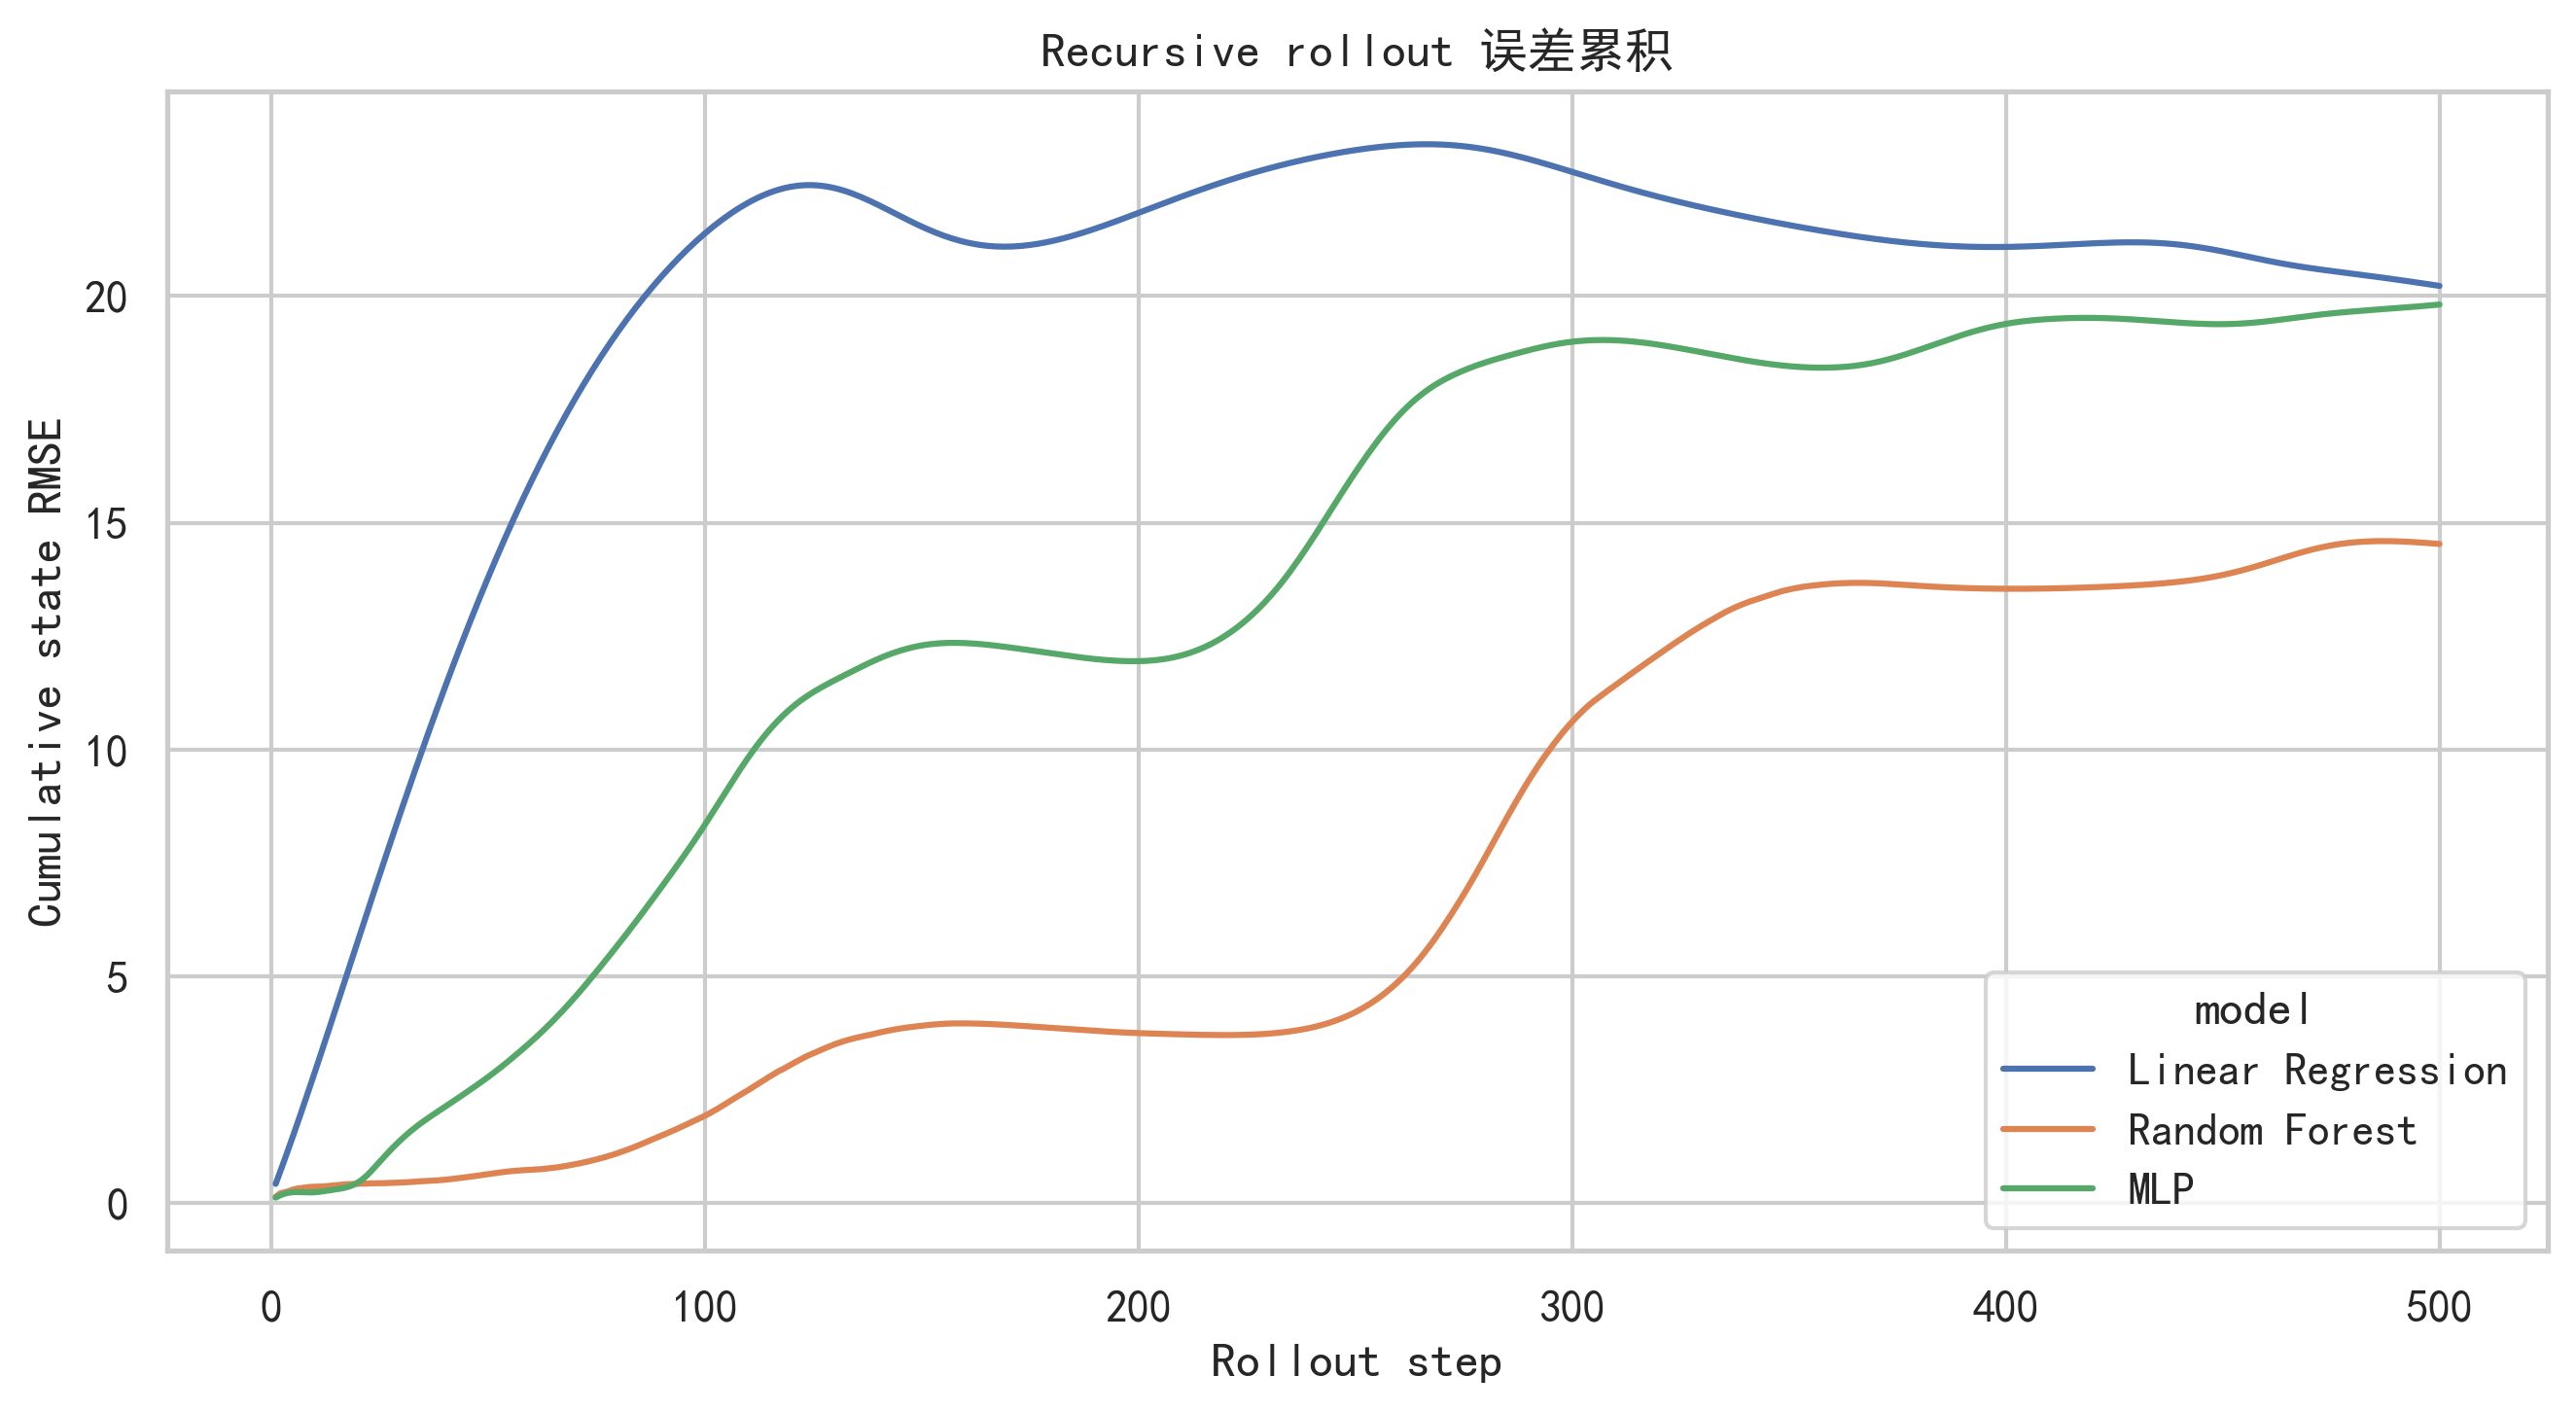
\includegraphics[width=0.86\textwidth]{figures/rollout_error.png}
\caption{递归多步预测中的误差累积曲线。与直接多步预测不同，rollout 会将模型自身误差反复输入下一步。}
\label{fig:rollout_error}
\end{figure}

图 \ref{fig:rollout_x} 展示了 rollout 中 $x(t)$ 的真实值与预测值对比。即使一步模型在短期预测上表现较好，连续递推后仍会逐渐偏离真实轨迹。

\begin{figure}[H]
\centering
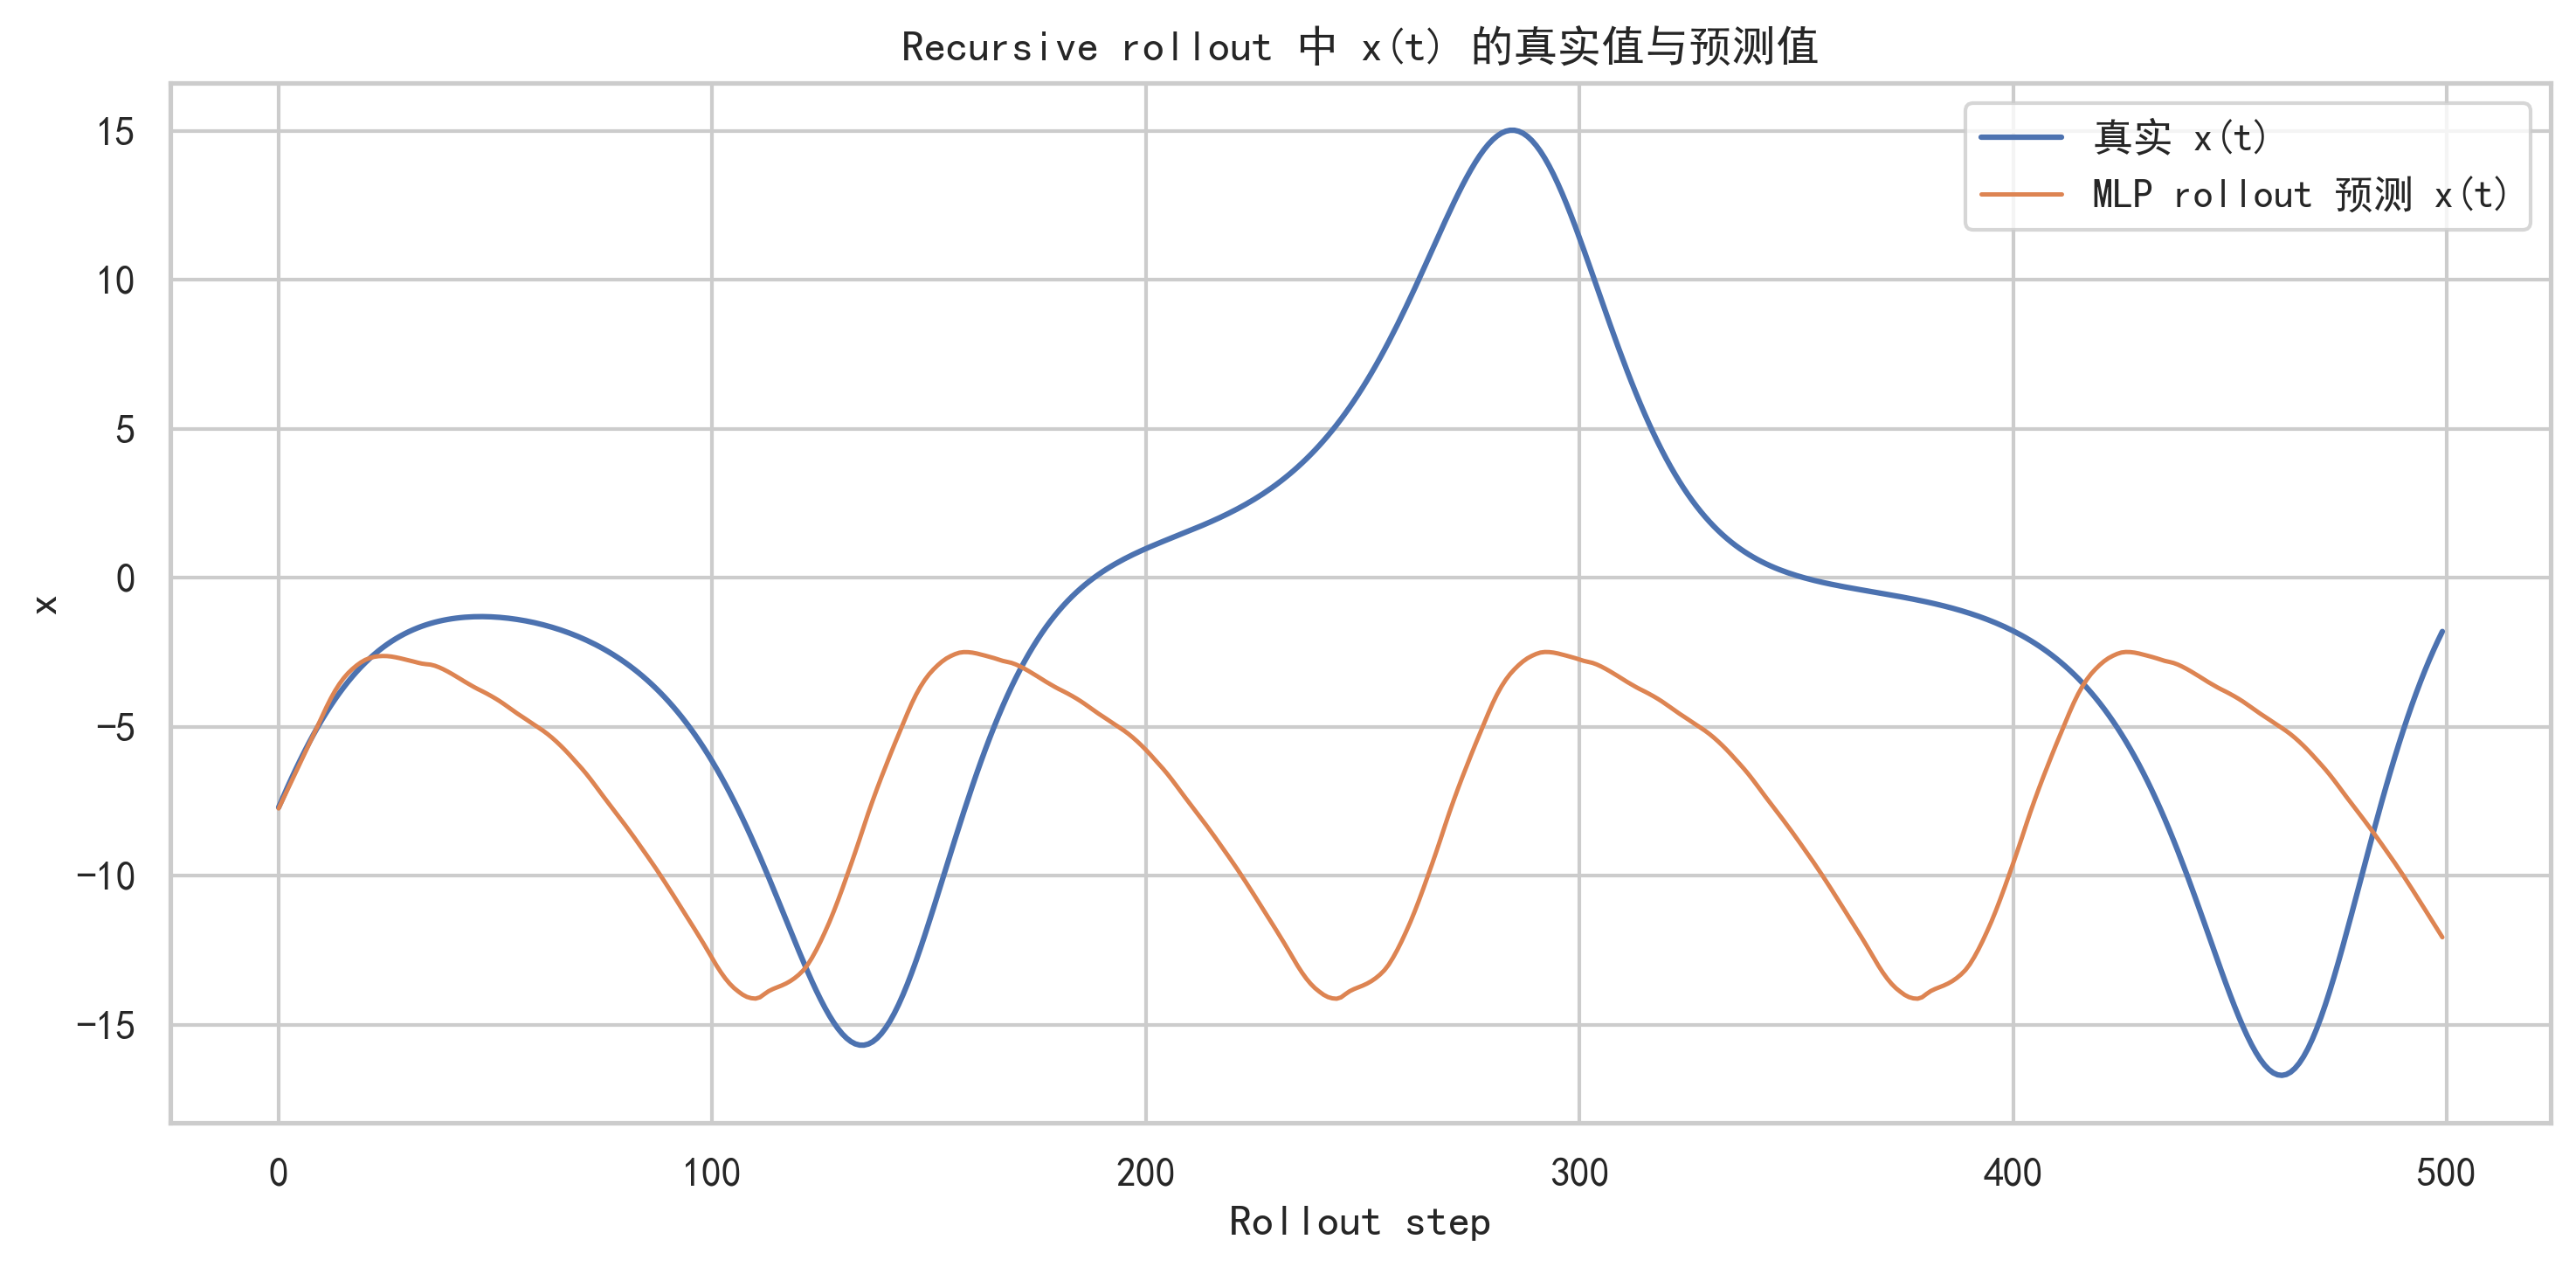
\includegraphics[width=0.86\textwidth]{figures/rollout_x_comparison.png}
\caption{递归多步预测中 $x(t)$ 的真实值与预测值对比}
\label{fig:rollout_x}
\end{figure}

图 \ref{fig:rollout_attractor} 从三维相空间角度比较真实轨迹与 rollout 预测轨迹。该图说明点预测误差的累积会进一步表现为相空间轨迹的偏移。

\begin{figure}[H]
\centering
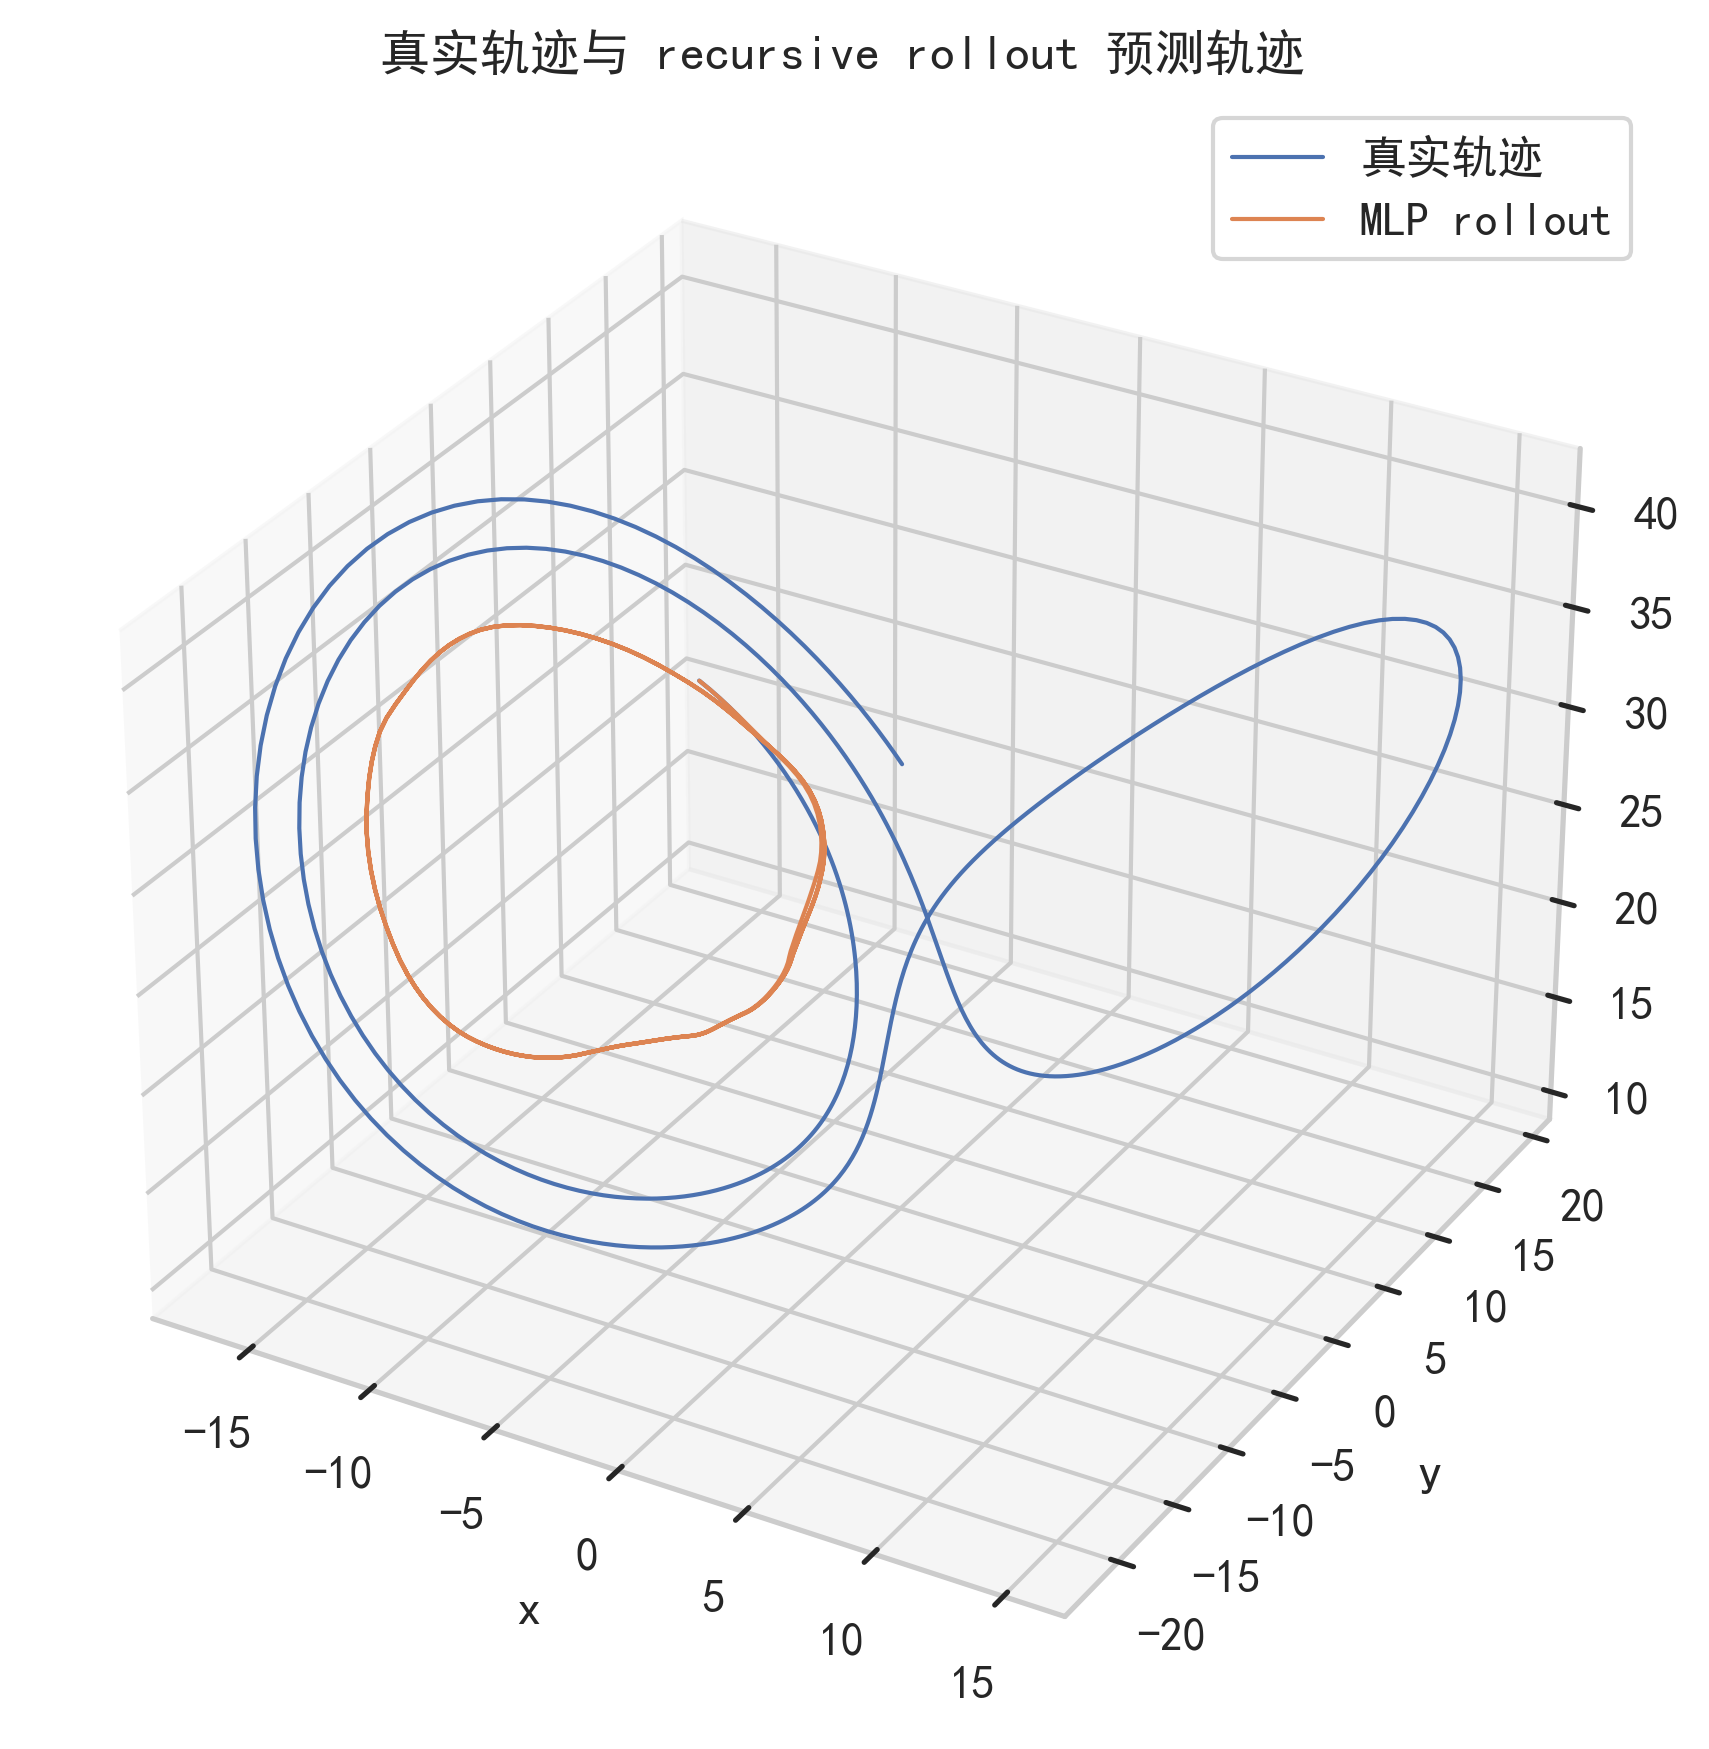
\includegraphics[width=0.78\textwidth]{figures/rollout_attractor.png}
\caption{真实轨迹与递归多步预测轨迹的三维对比}
\label{fig:rollout_attractor}
\end{figure}

\subsection{初始条件泛化（initial condition generalization）}

为了测试模型是否只是拟合同一条轨迹，本文保持模型训练数据主要来自初始条件 $(1,1,1)$，然后直接测试其他初始条件生成的轨迹，不进行重新训练。测试初始条件包括 $(1.01,1,1)$、$(1.1,1,1)$、$(-5,5,20)$ 和 $(10,10,10)$。

图 \ref{fig:ic_rmse} 展示了不同初始条件下的状态 RMSE。图中 IC1--IC4 分别对应 $(1.01,1,1)$、$(1.1,1,1)$、$(-5,5,20)$ 和 $(10,10,10)$。结果表明，非线性模型在新初值轨迹上仍明显优于 Persistence 和 Linear Regression，但误差水平会随初始条件和轨迹分布变化而波动。这说明模型具有一定局部泛化能力，但其泛化仍受到训练轨迹覆盖范围限制。

\begin{figure}[H]
\centering
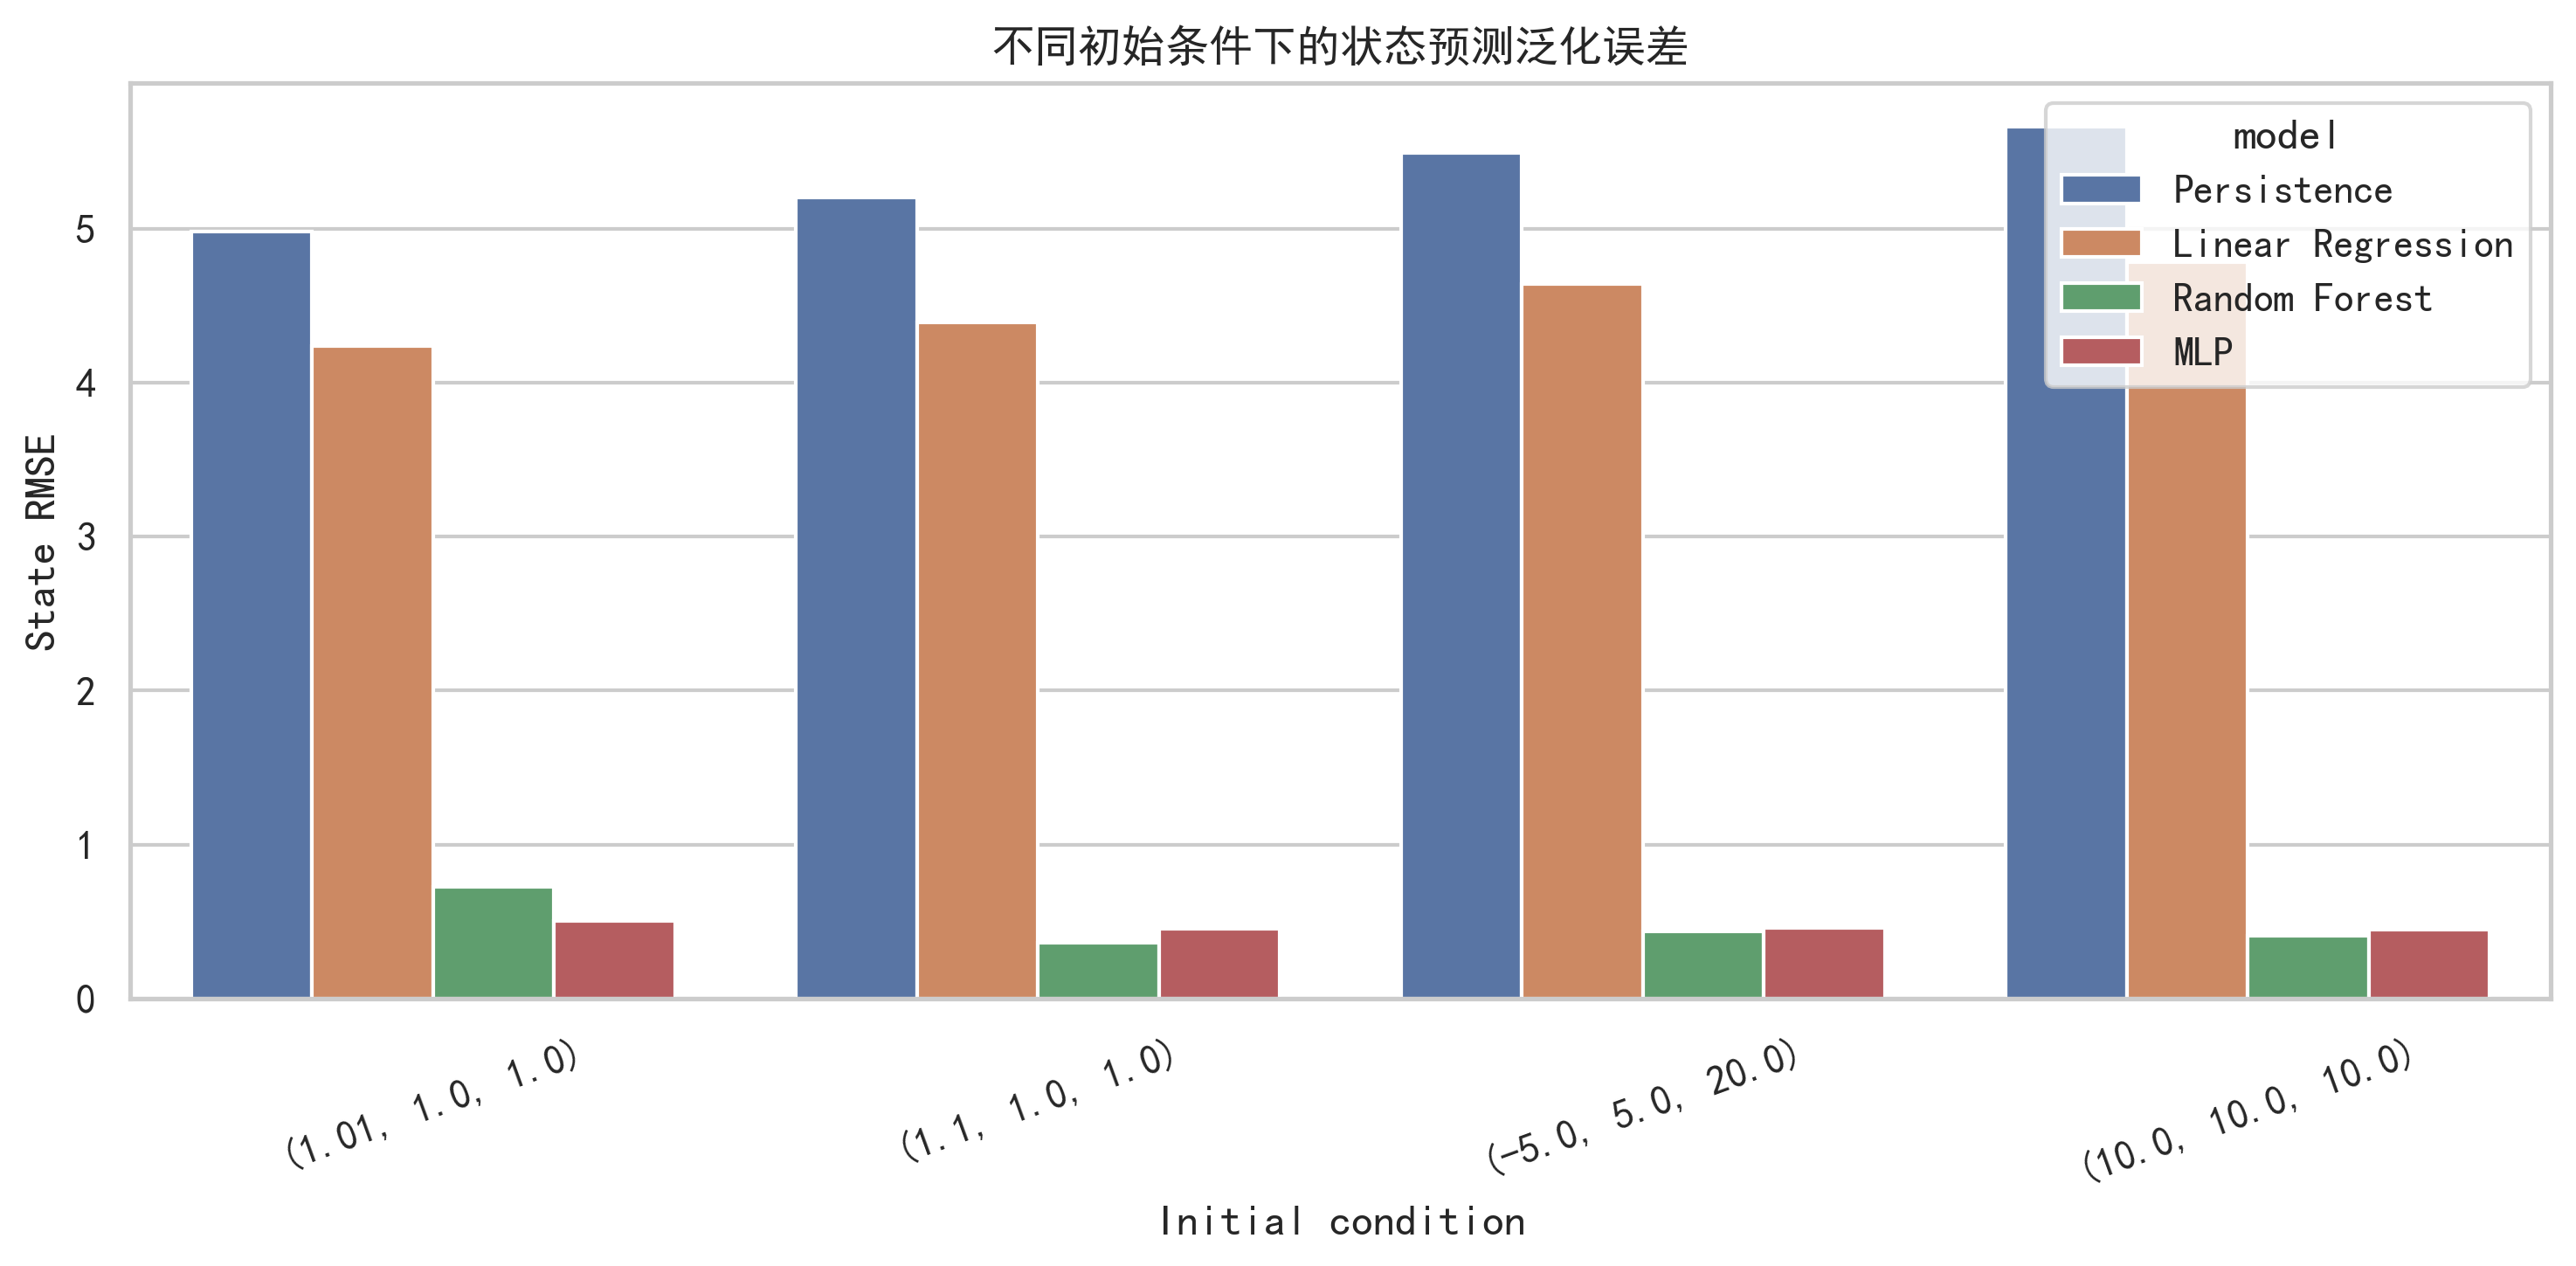
\includegraphics[width=0.88\textwidth]{figures/initial_condition_rmse.png}
\caption{不同初始条件下的状态预测泛化误差。IC1--IC4 为四组测试初始条件的简写。}
\label{fig:ic_rmse}
\end{figure}

\subsection{残差状态转移建模与模型增强}

为了进一步分析什么样的模型结构更适合 Lorenz 系统的连续状态转移映射，本文加入输出标准化、Residual MLP、MLP 结构和激活函数消融，以及 ESN 对照。表 \ref{tab:model_enhancement} 只展示代表性结果，完整消融结果见 \texttt{results/model\_enhancement\_results.csv}。

\begin{table}[H]
\centering
\caption{模型增强实验的代表性结果。表中保留关键模型与预测步长，用于说明 Residual MLP 的中短期优势和长步长退化。}
\label{tab:model_enhancement}
\begin{tabular}{rlcc}
\toprule
Horizon & 模型 & State RMSE & $R^2_{mean}$ \\
\midrule
10 & 原始 MLP & 0.4572 & 0.9991 \\
10 & Residual MLP ReLU 64-64-64 & 0.0772 & 0.99997 \\
10 & ESN residual & 0.4566 & 0.9991 \\
100 & 原始 MLP & 2.2369 & 0.9781 \\
100 & Residual MLP ReLU 64-64-64 & 1.4133 & 0.9913 \\
100 & ESN residual & 76.9877 & -26.0032 \\
500 & 原始 MLP & 13.6858 & 0.1591 \\
500 & Residual MLP ReLU 64-64 & 13.8243 & 0.1417 \\
500 & Random Forest 基线 & 12.7868 & 0.2607 \\
\bottomrule
\end{tabular}
\end{table}

图 \ref{fig:model_enhancement} 展示了不同增强模型在 $k=10$、100、500 下的状态 RMSE。为避免 ESN 在长步长上的极端误差压缩其他模型的可读性，该图只绘制主要 MLP 变体和基线模型，ESN 结果保留在表格和文字讨论中。结果表明，输出标准化和残差学习在短期和中期预测中明显改善 MLP 表现；其中更深的 ReLU Residual MLP 在 $k=10$ 和 $k=100$ 上表现最好。但当 $k$ 增大到 500 时，各类 MLP 都出现明显退化，Random Forest 反而保持相对较低误差。这说明模型结构改进可以扩大可预测时间窗，但不能消除混沌系统长期预测困难。

\begin{figure}[H]
\centering
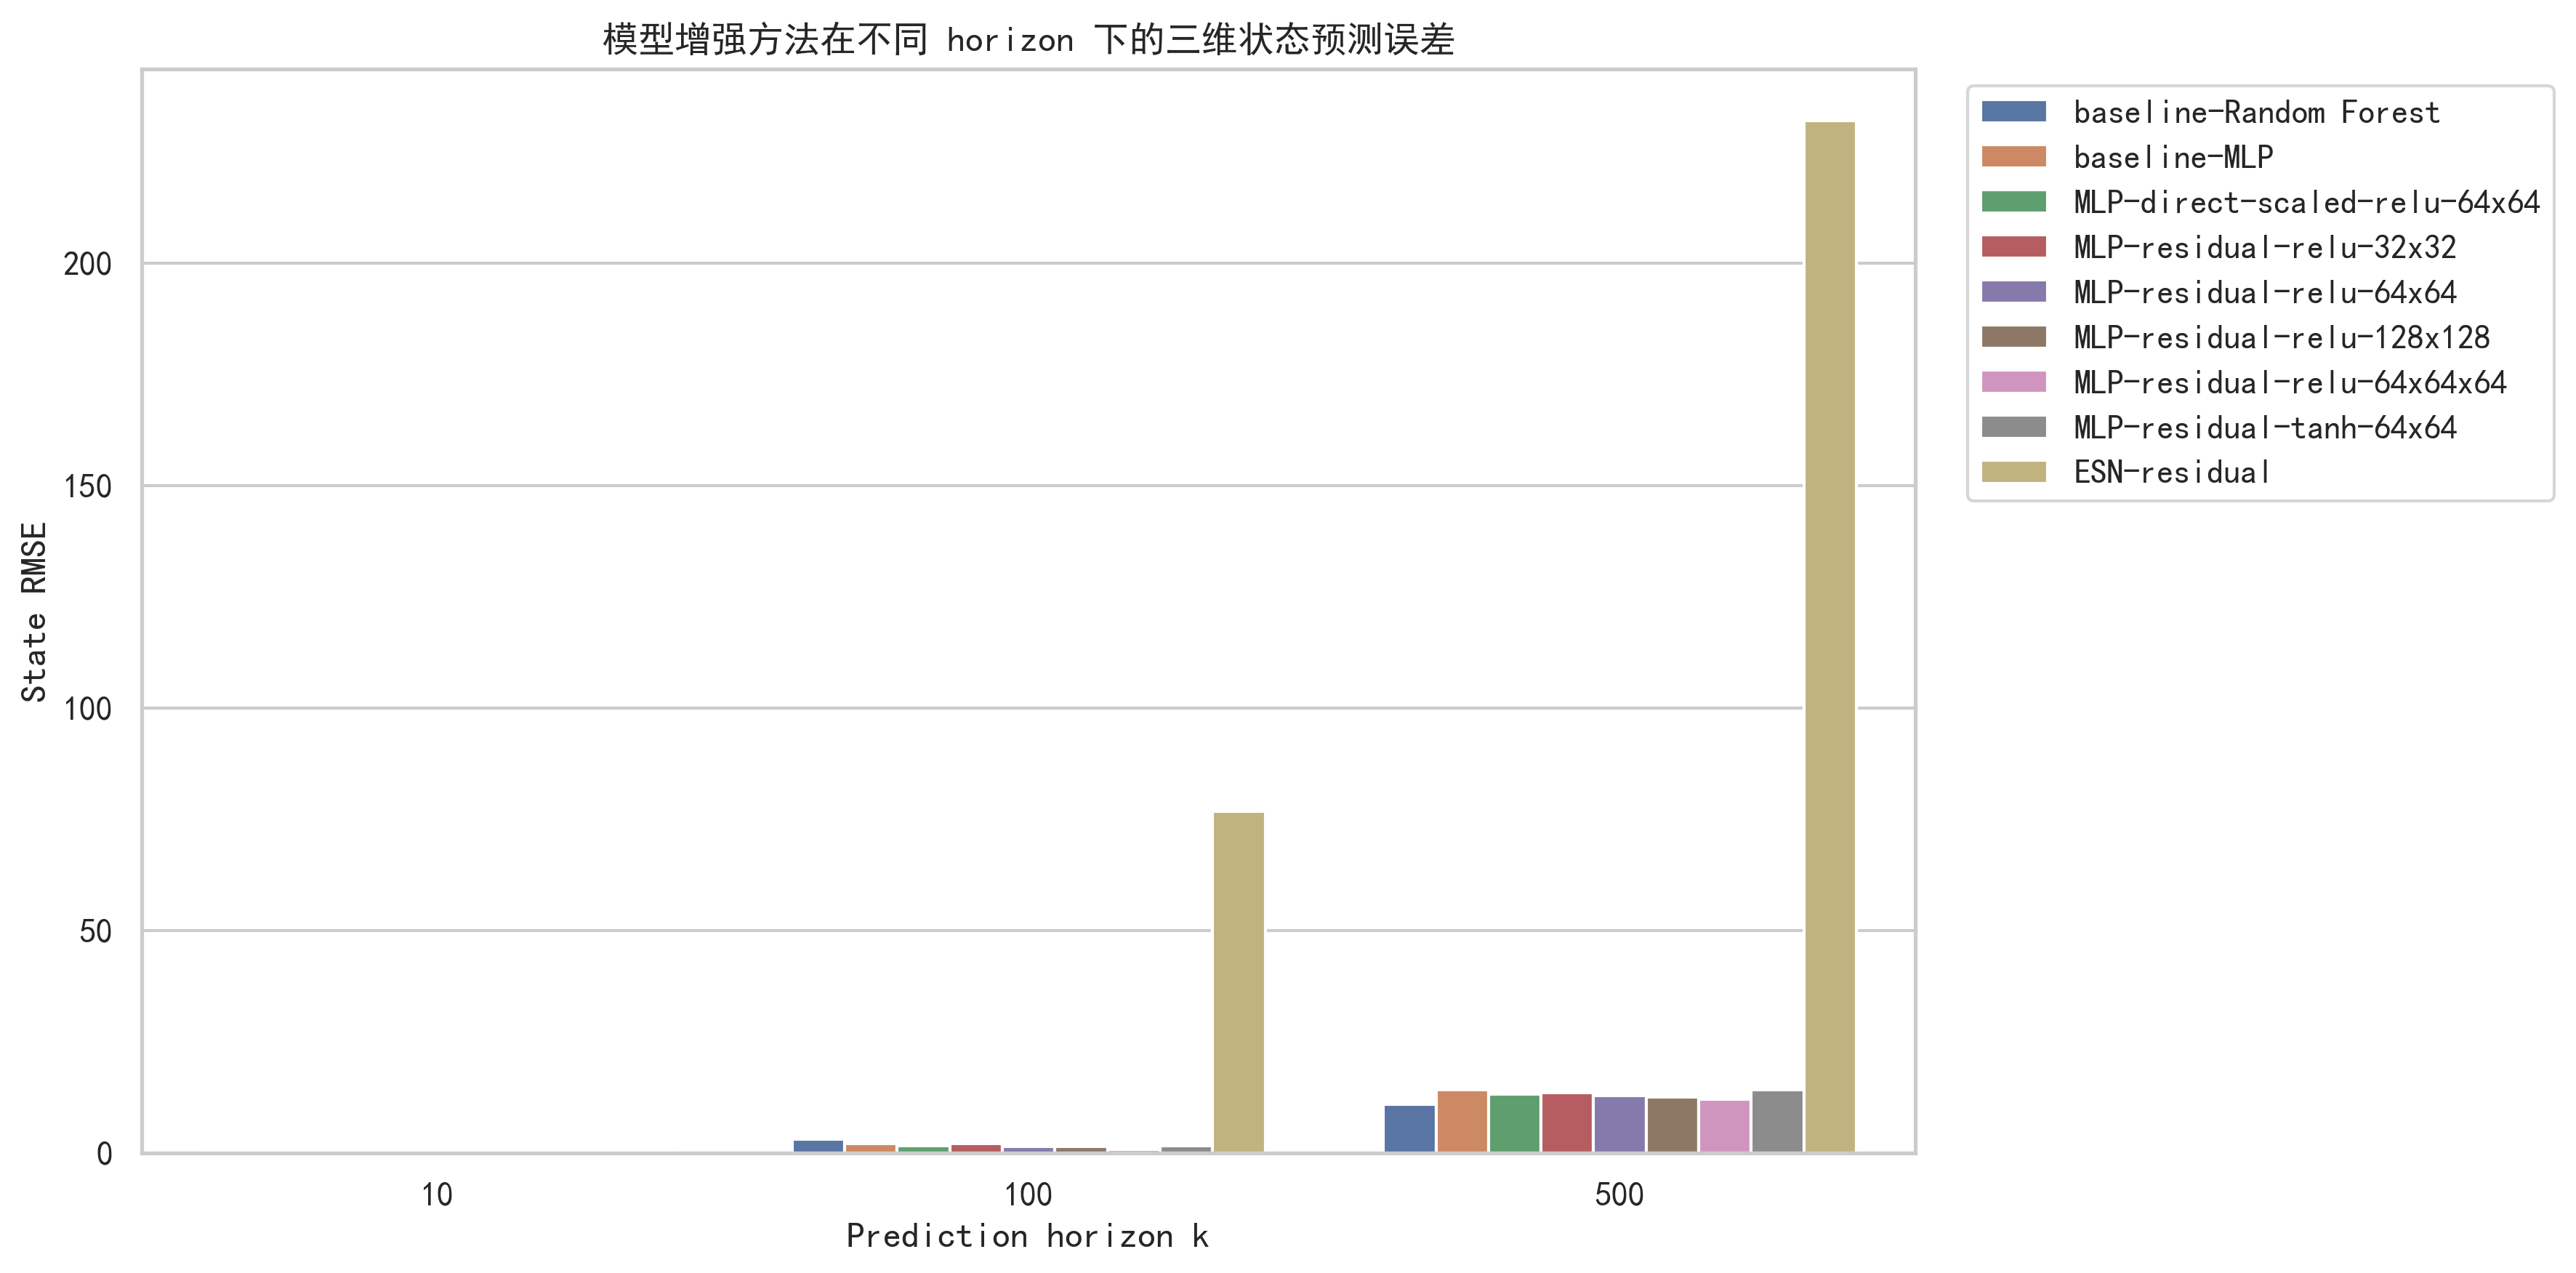
\includegraphics[width=0.95\textwidth]{figures/model_enhancement_horizon_rmse.png}
\caption{Residual MLP 与输出标准化在不同预测步长下的对比。ESN 因长步长误差过大未绘入该图，以保持主要模型差异的可读性。}
\label{fig:model_enhancement}
\end{figure}

图 \ref{fig:enhanced_rollout_error} 展示了增强模型在 500 步递归多步预测中的误差。Residual MLP tanh 64-64 的累计状态 RMSE 约为 10.7975，优于原始 MLP rollout 的 18.0711；ESN residual 的累计状态 RMSE 约为 14.7144，表现中等但提供了动力系统时间序列模型视角。

\begin{figure}[H]
\centering
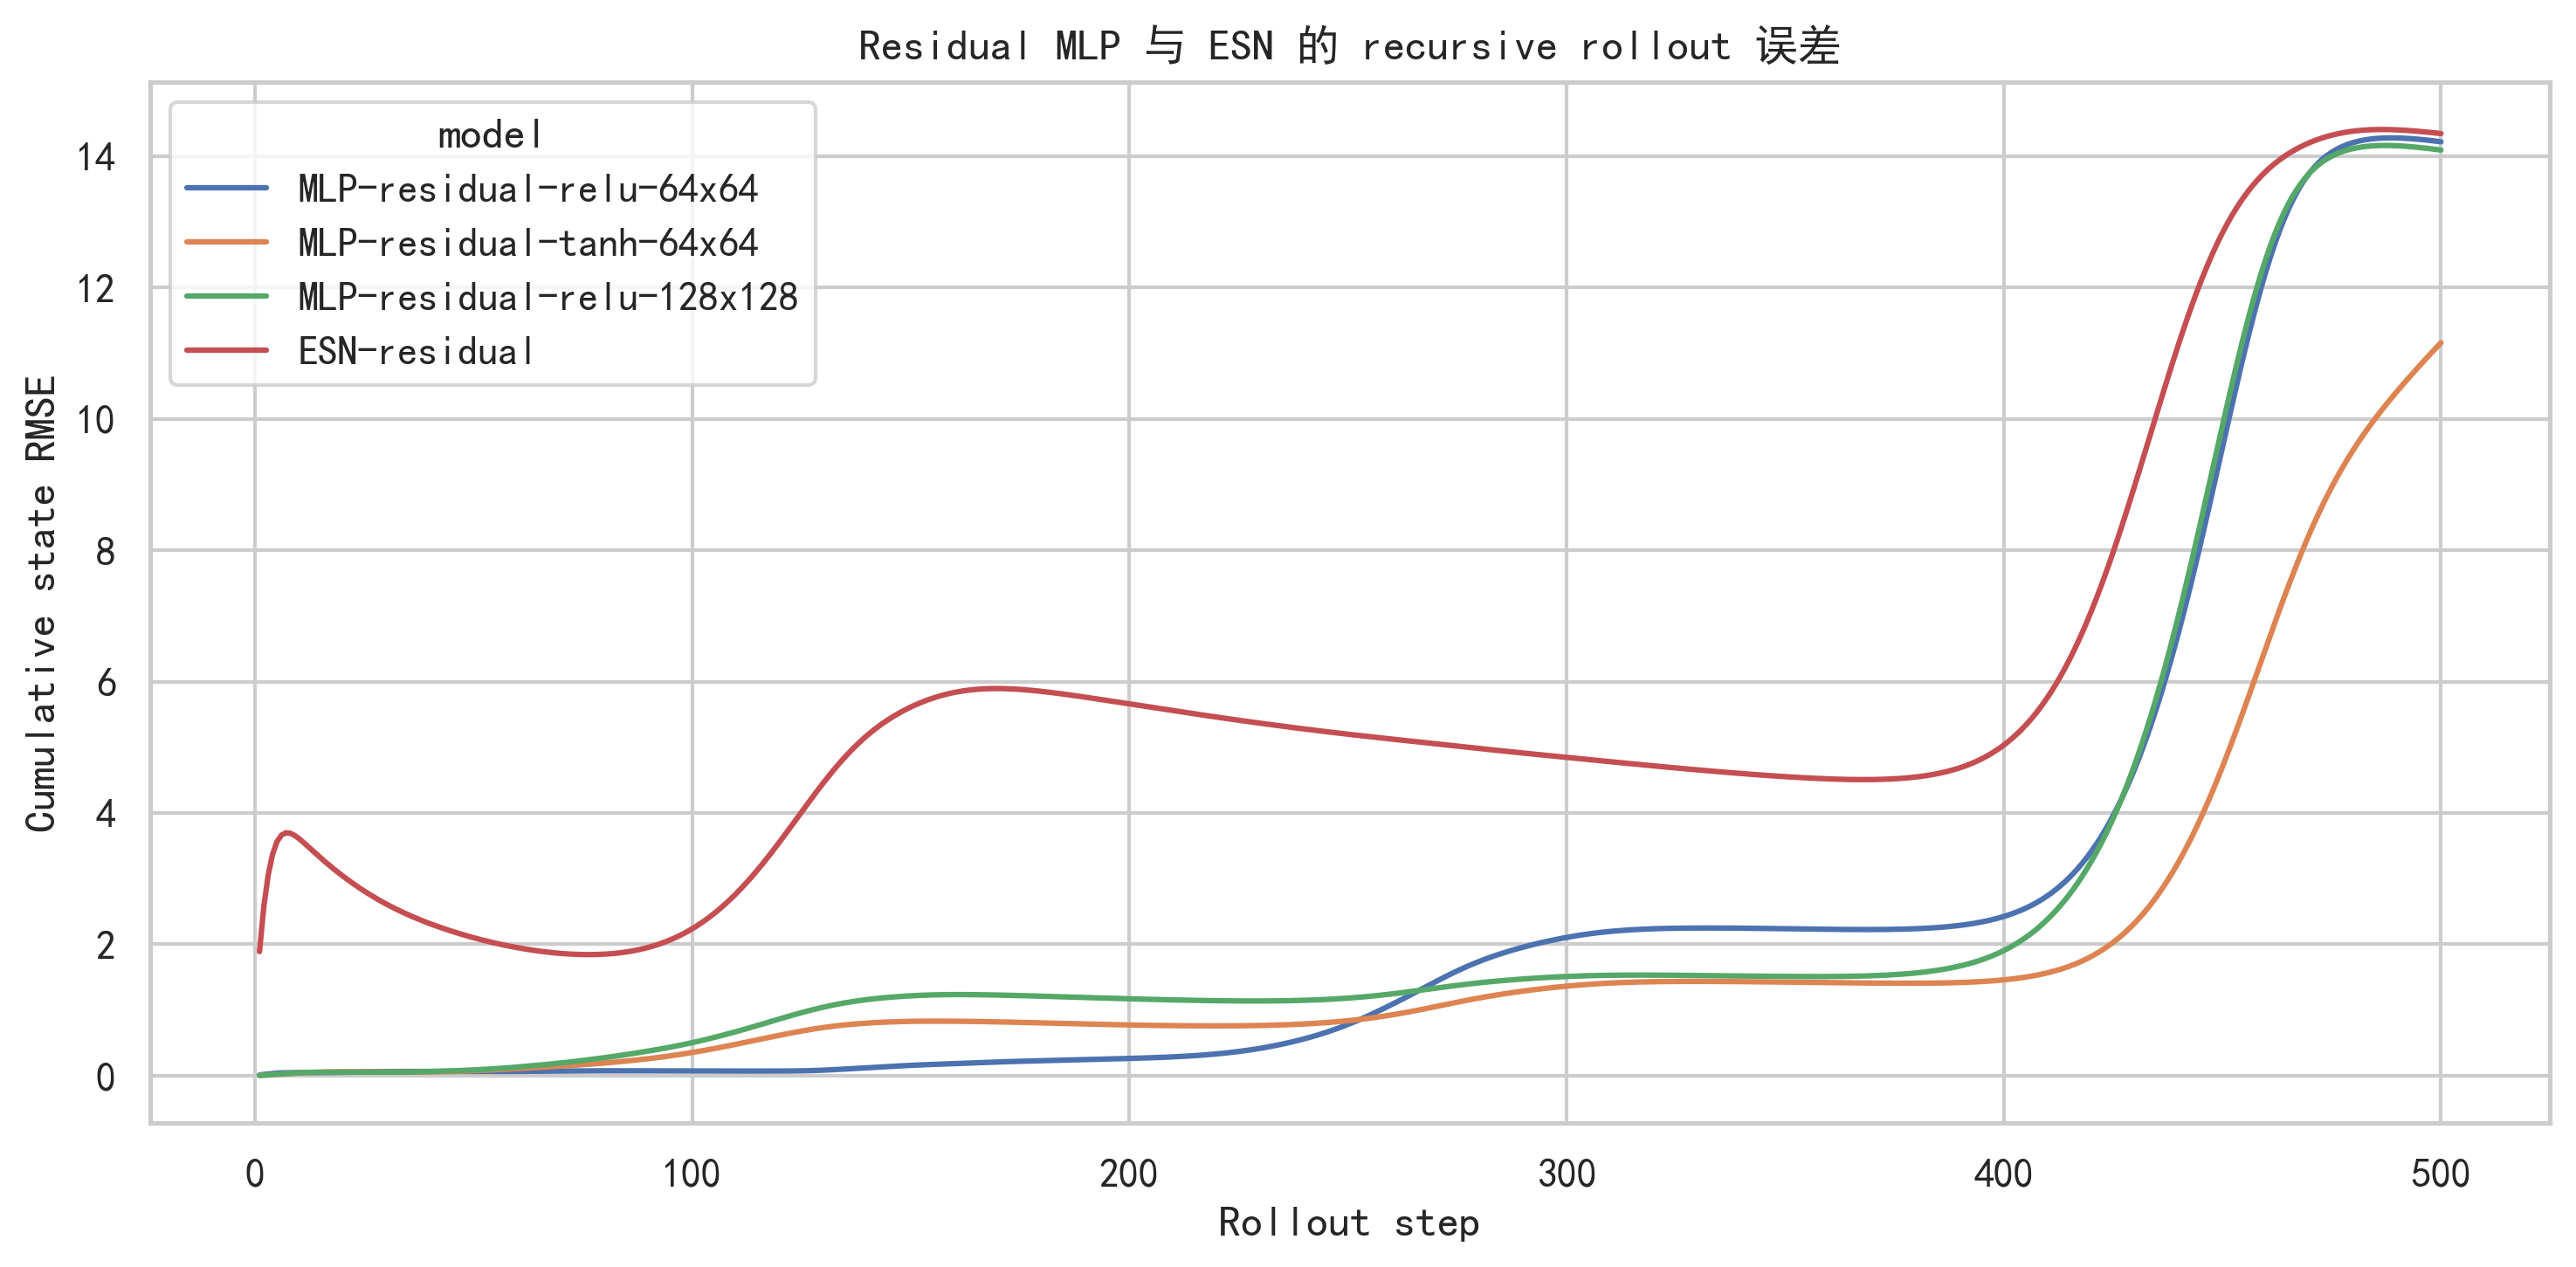
\includegraphics[width=0.88\textwidth]{figures/enhanced_rollout_error.png}
\caption{增强模型递归多步预测误差曲线}
\label{fig:enhanced_rollout_error}
\end{figure}

\begin{figure}[H]
\centering
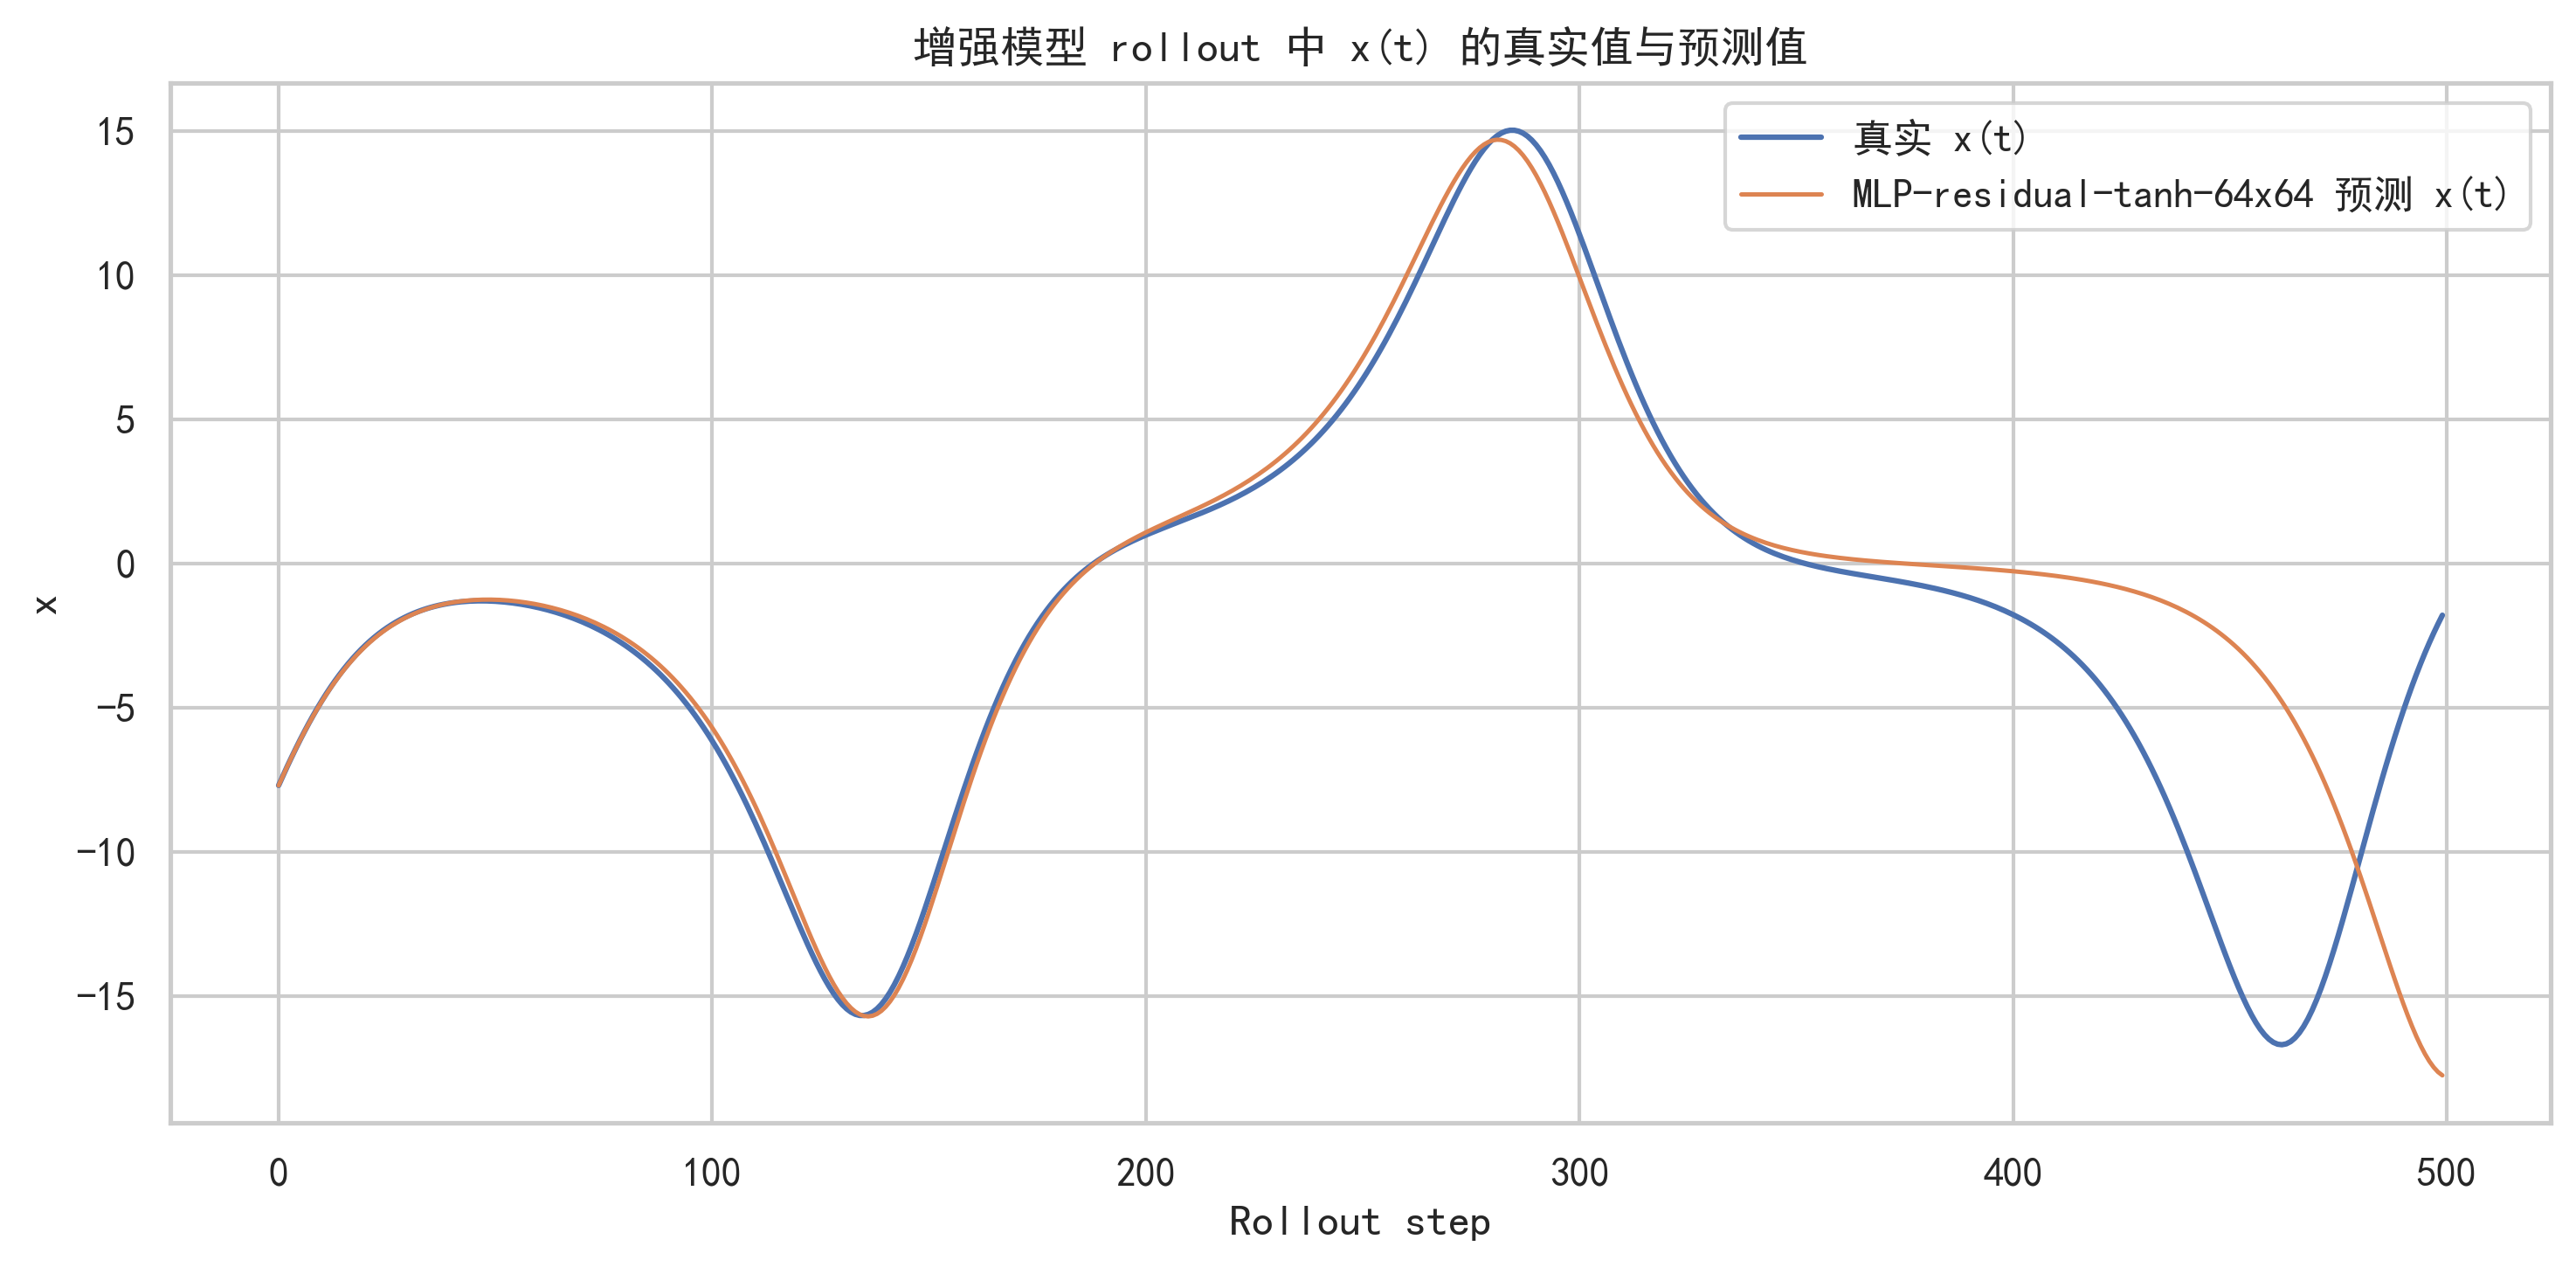
\includegraphics[width=0.88\textwidth]{figures/enhanced_rollout_x_comparison.png}
\caption{增强模型递归多步预测中 $x(t)$ 的真实值与预测值对比}
\label{fig:enhanced_rollout_x}
\end{figure}

\subsection{SINDy 稀疏动力学识别}

前述模型主要回答“能否预测未来状态”，但没有直接说明模型是否理解了 Lorenz 系统的方程结构。表 \ref{tab:sindy_coefficients} 展示了 SINDy 从轨迹数据中恢复出的非零项。可以看到，恢复结果接近真实 Lorenz 方程：$dx/dt$ 主要由 $-x$ 和 $y$ 控制，$dy/dt$ 包含 $x$、$y$ 和 $xz$，$dz/dt$ 包含 $xy$ 和 $z$。这说明数据中确实包含可被稀疏方法识别的动力学结构。

\begin{table}[H]
\centering
\caption{SINDy 恢复的 Lorenz 方程主要非零系数}
\label{tab:sindy_coefficients}
\begin{tabular}{lccc}
\toprule
候选项 & $dx/dt$ & $dy/dt$ & $dz/dt$ \\
\midrule
$x$ & -9.9943 & 27.9517 & 0 \\
$y$ & 9.9943 & -0.9906 & 0 \\
$z$ & 0 & 0 & -2.6646 \\
$xy$ & 0 & 0 & 0.9992 \\
$xz$ & 0 & -0.9986 & 0 \\
\bottomrule
\end{tabular}
\end{table}

\begin{figure}[H]
\centering
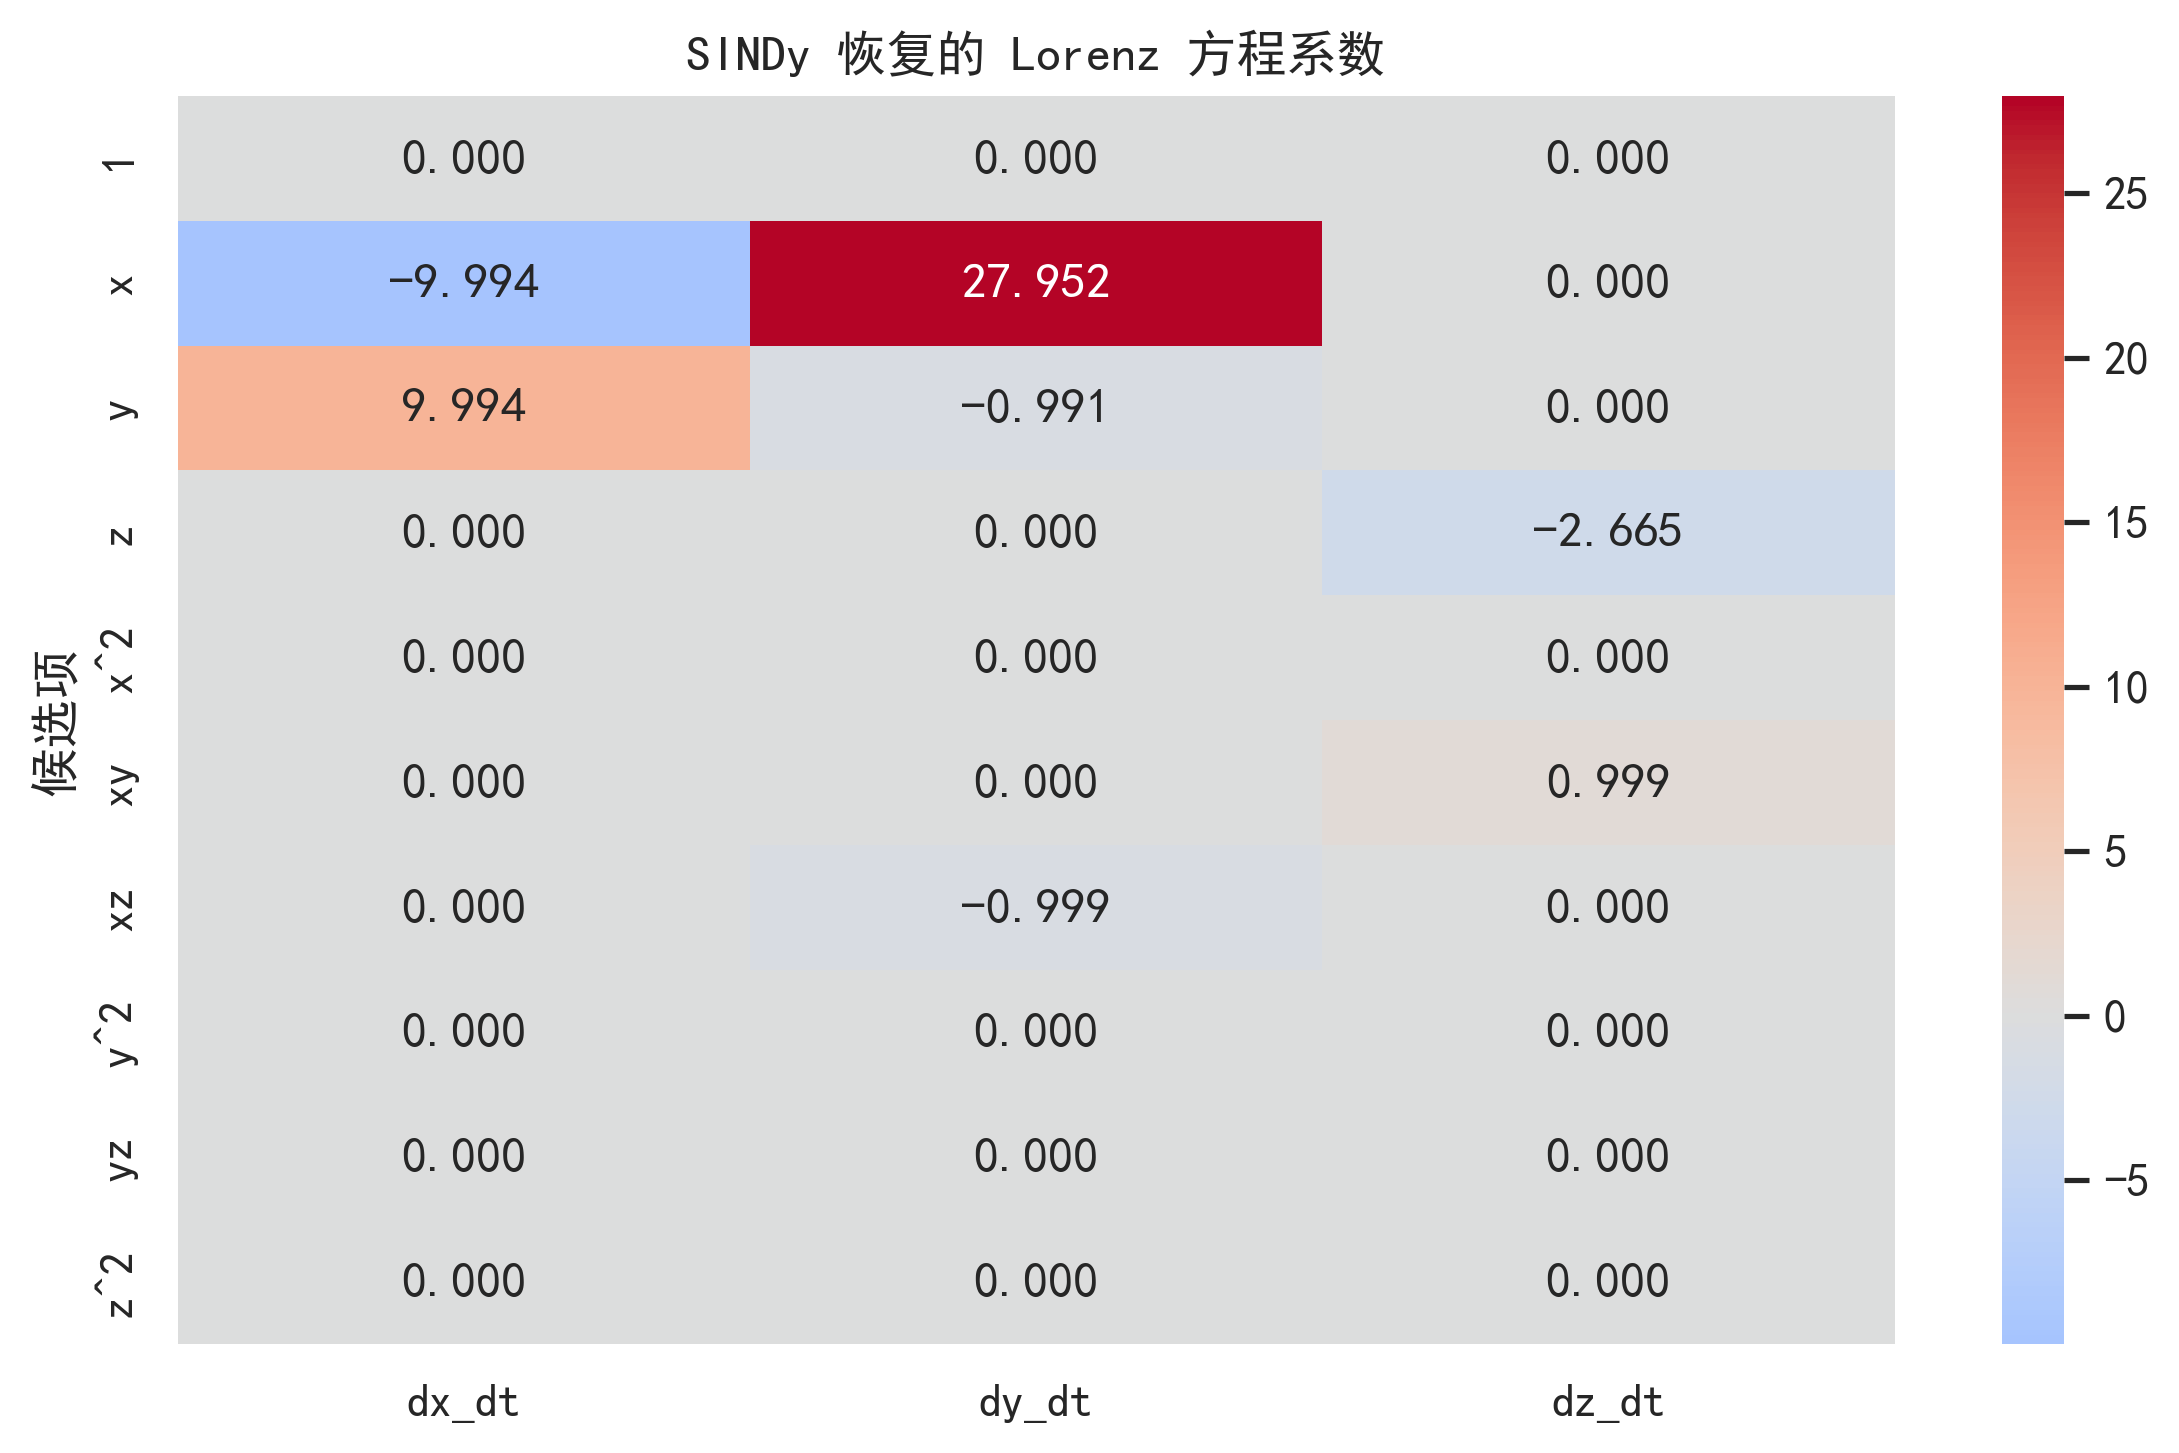
\includegraphics[width=0.82\textwidth]{figures/sindy_coefficients.png}
\caption{SINDy 恢复的 Lorenz 方程系数热力图}
\label{fig:sindy_coefficients}
\end{figure}

图 \ref{fig:sindy_rollout} 展示了 SINDy 恢复方程的 500 步 rollout。由于恢复方程接近真实方程，短期轨迹能够较好贴合真实 $x(t)$；但由于 Lorenz 系统本身对误差敏感，即使方程系数只有很小偏差，长期逐点轨迹仍可能逐渐分离。因此，SINDy 的价值主要在于恢复动力学结构，而不是保证无限长期逐点预测。

\begin{figure}[H]
\centering
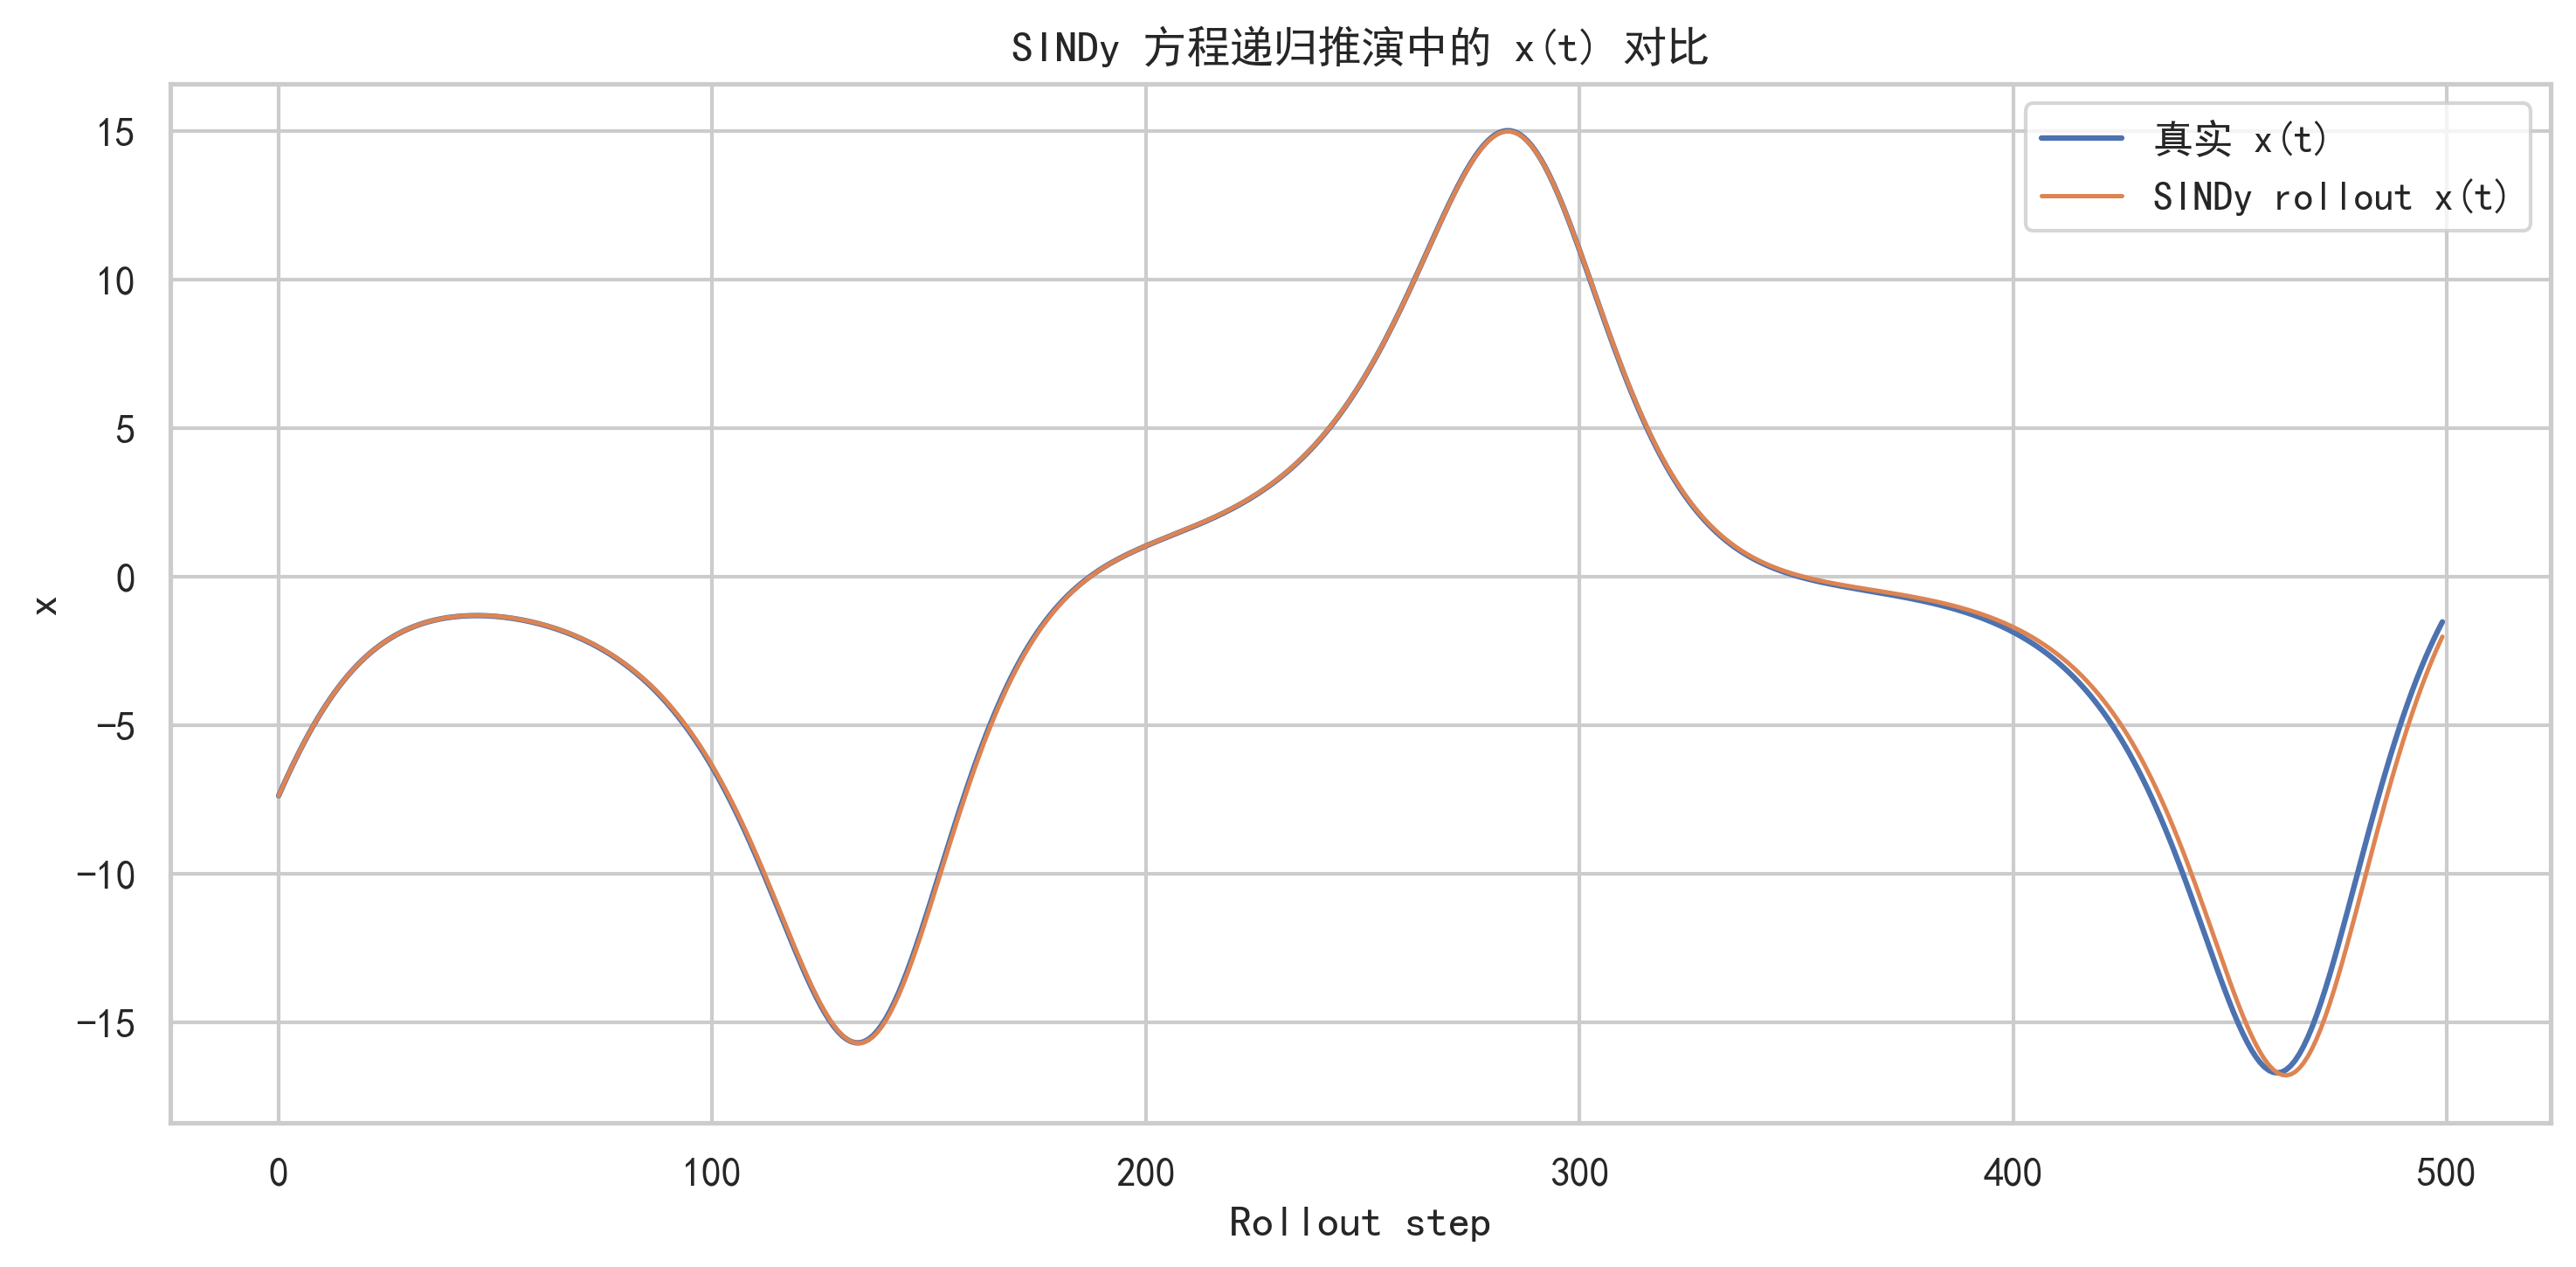
\includegraphics[width=0.88\textwidth]{figures/sindy_rollout_x_comparison.png}
\caption{SINDy 恢复方程递归推演中 $x(t)$ 的真实值与预测值对比}
\label{fig:sindy_rollout}
\end{figure}

\subsection{物理-机器学习混合修正}

为了模拟真实科学建模中“已有物理模型但参数有偏”的情况，本文构造了一个不完美 Lorenz 模型，将 $\rho$ 从真实值 28 改为 26。表 \ref{tab:hybrid_metrics} 比较了一步预测误差。可以看到，不完美物理模型的一步状态 RMSE 为 0.0786；pure ML residual MLP 可降至 0.0102；Hybrid RF 和 Hybrid MLP 通过学习物理模型残差，将一步状态 RMSE 进一步降至 0.0003 和 0.0006。

\begin{table}[H]
\centering
\caption{不完美物理模型、Pure ML 与 Hybrid correction 的一步状态预测结果}
\label{tab:hybrid_metrics}
\begin{tabular}{lcc}
\toprule
模型 & State RMSE & $R^2_{mean}$ \\
\midrule
Imperfect physics & 0.0786 & 0.99997 \\
Pure ML Residual MLP & 0.0102 & 0.9999996 \\
Hybrid RF & 0.0003 & 0.9999999996 \\
Hybrid MLP & 0.0006 & 0.9999999986 \\
\bottomrule
\end{tabular}
\end{table}

\begin{figure}[H]
\centering
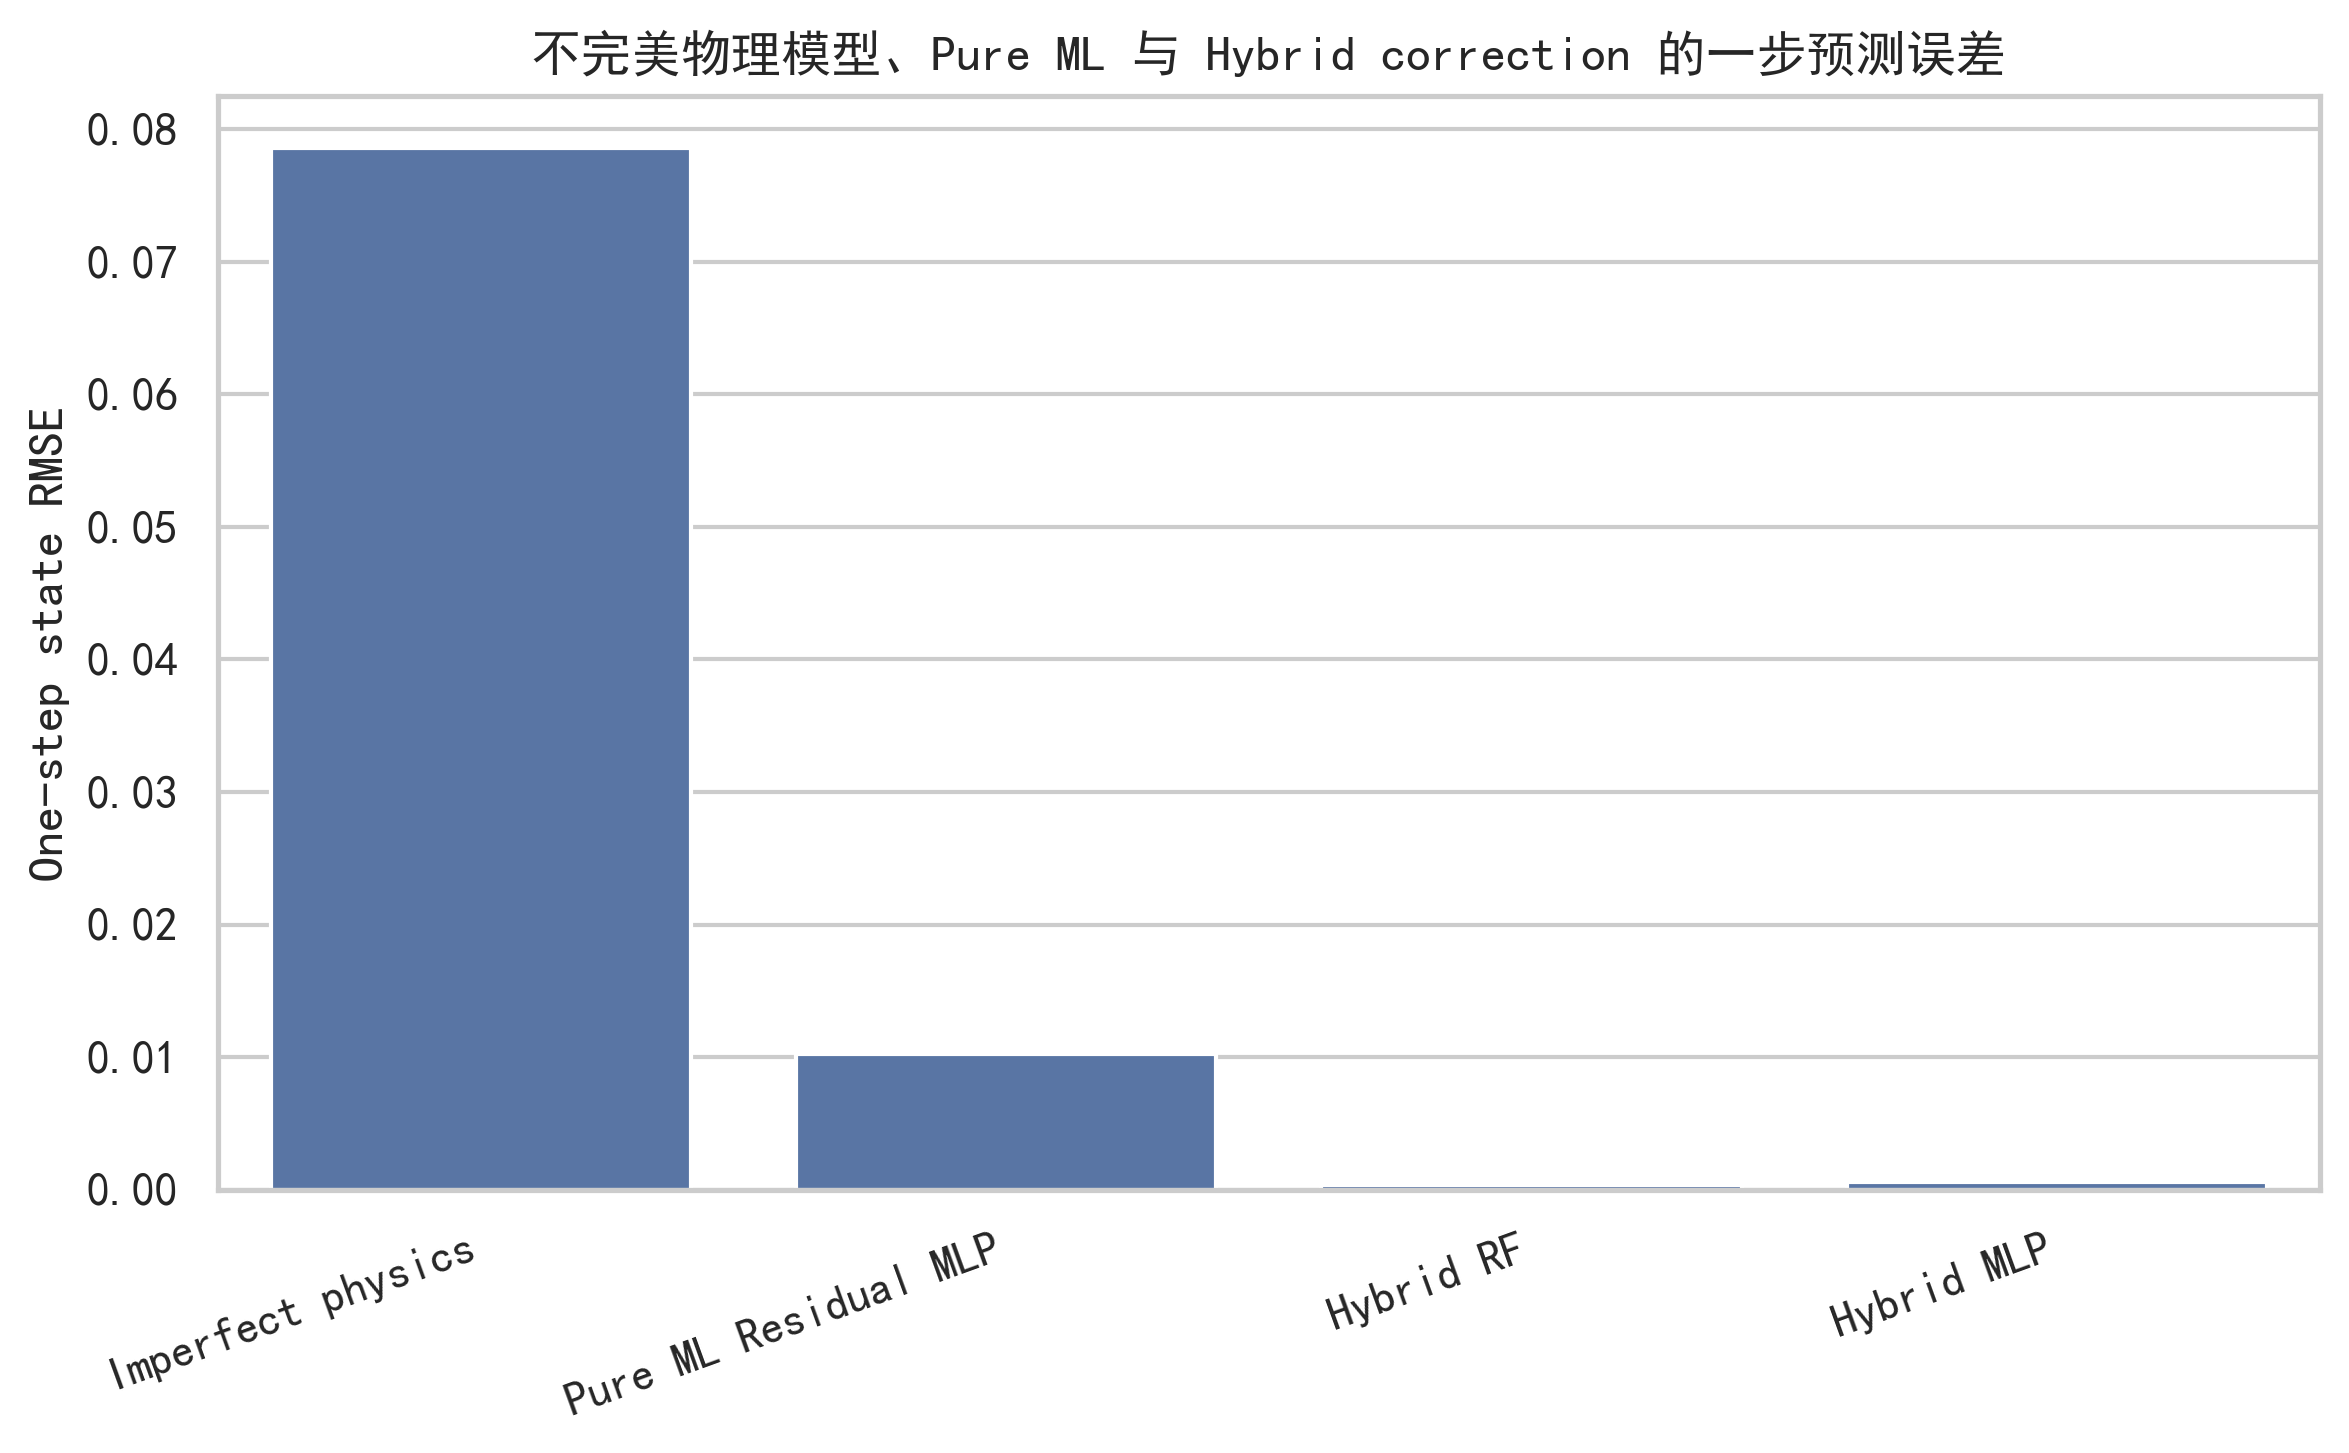
\includegraphics[width=0.82\textwidth]{figures/hybrid_one_step_metrics.png}
\caption{不完美物理模型、Pure ML 与 Hybrid correction 的一步状态 RMSE 对比}
\label{fig:hybrid_one_step}
\end{figure}

在 500 步 recursive rollout 中，Hybrid correction 的优势更明显。表 \ref{tab:valid_prediction_time} 使用状态误差阈值 5.5234 计算有效预测时间，并换算为 Lyapunov time。Imperfect physics 约在 0.35 个 Lyapunov time 后失效；Pure ML residual MLP 可维持约 1.86 个 Lyapunov time；Hybrid RF 和 Hybrid MLP 在 500 步窗口内均未超过阈值，对应至少 2.25 个 Lyapunov time。

\begin{table}[H]
\centering
\caption{500 步 rollout 中的有效预测时间}
\label{tab:valid_prediction_time}
\begin{tabular}{lccc}
\toprule
模型 & 有效步数 & 物理时间 & Lyapunov time \\
\midrule
Imperfect physics & 77 & 0.3850 & 0.3465 \\
Pure ML Residual MLP & 413 & 2.0652 & 1.8587 \\
Hybrid RF & 500 & 2.5003 & 2.2502 \\
Hybrid MLP & 500 & 2.5003 & 2.2502 \\
\bottomrule
\end{tabular}
\end{table}

\begin{figure}[H]
\centering
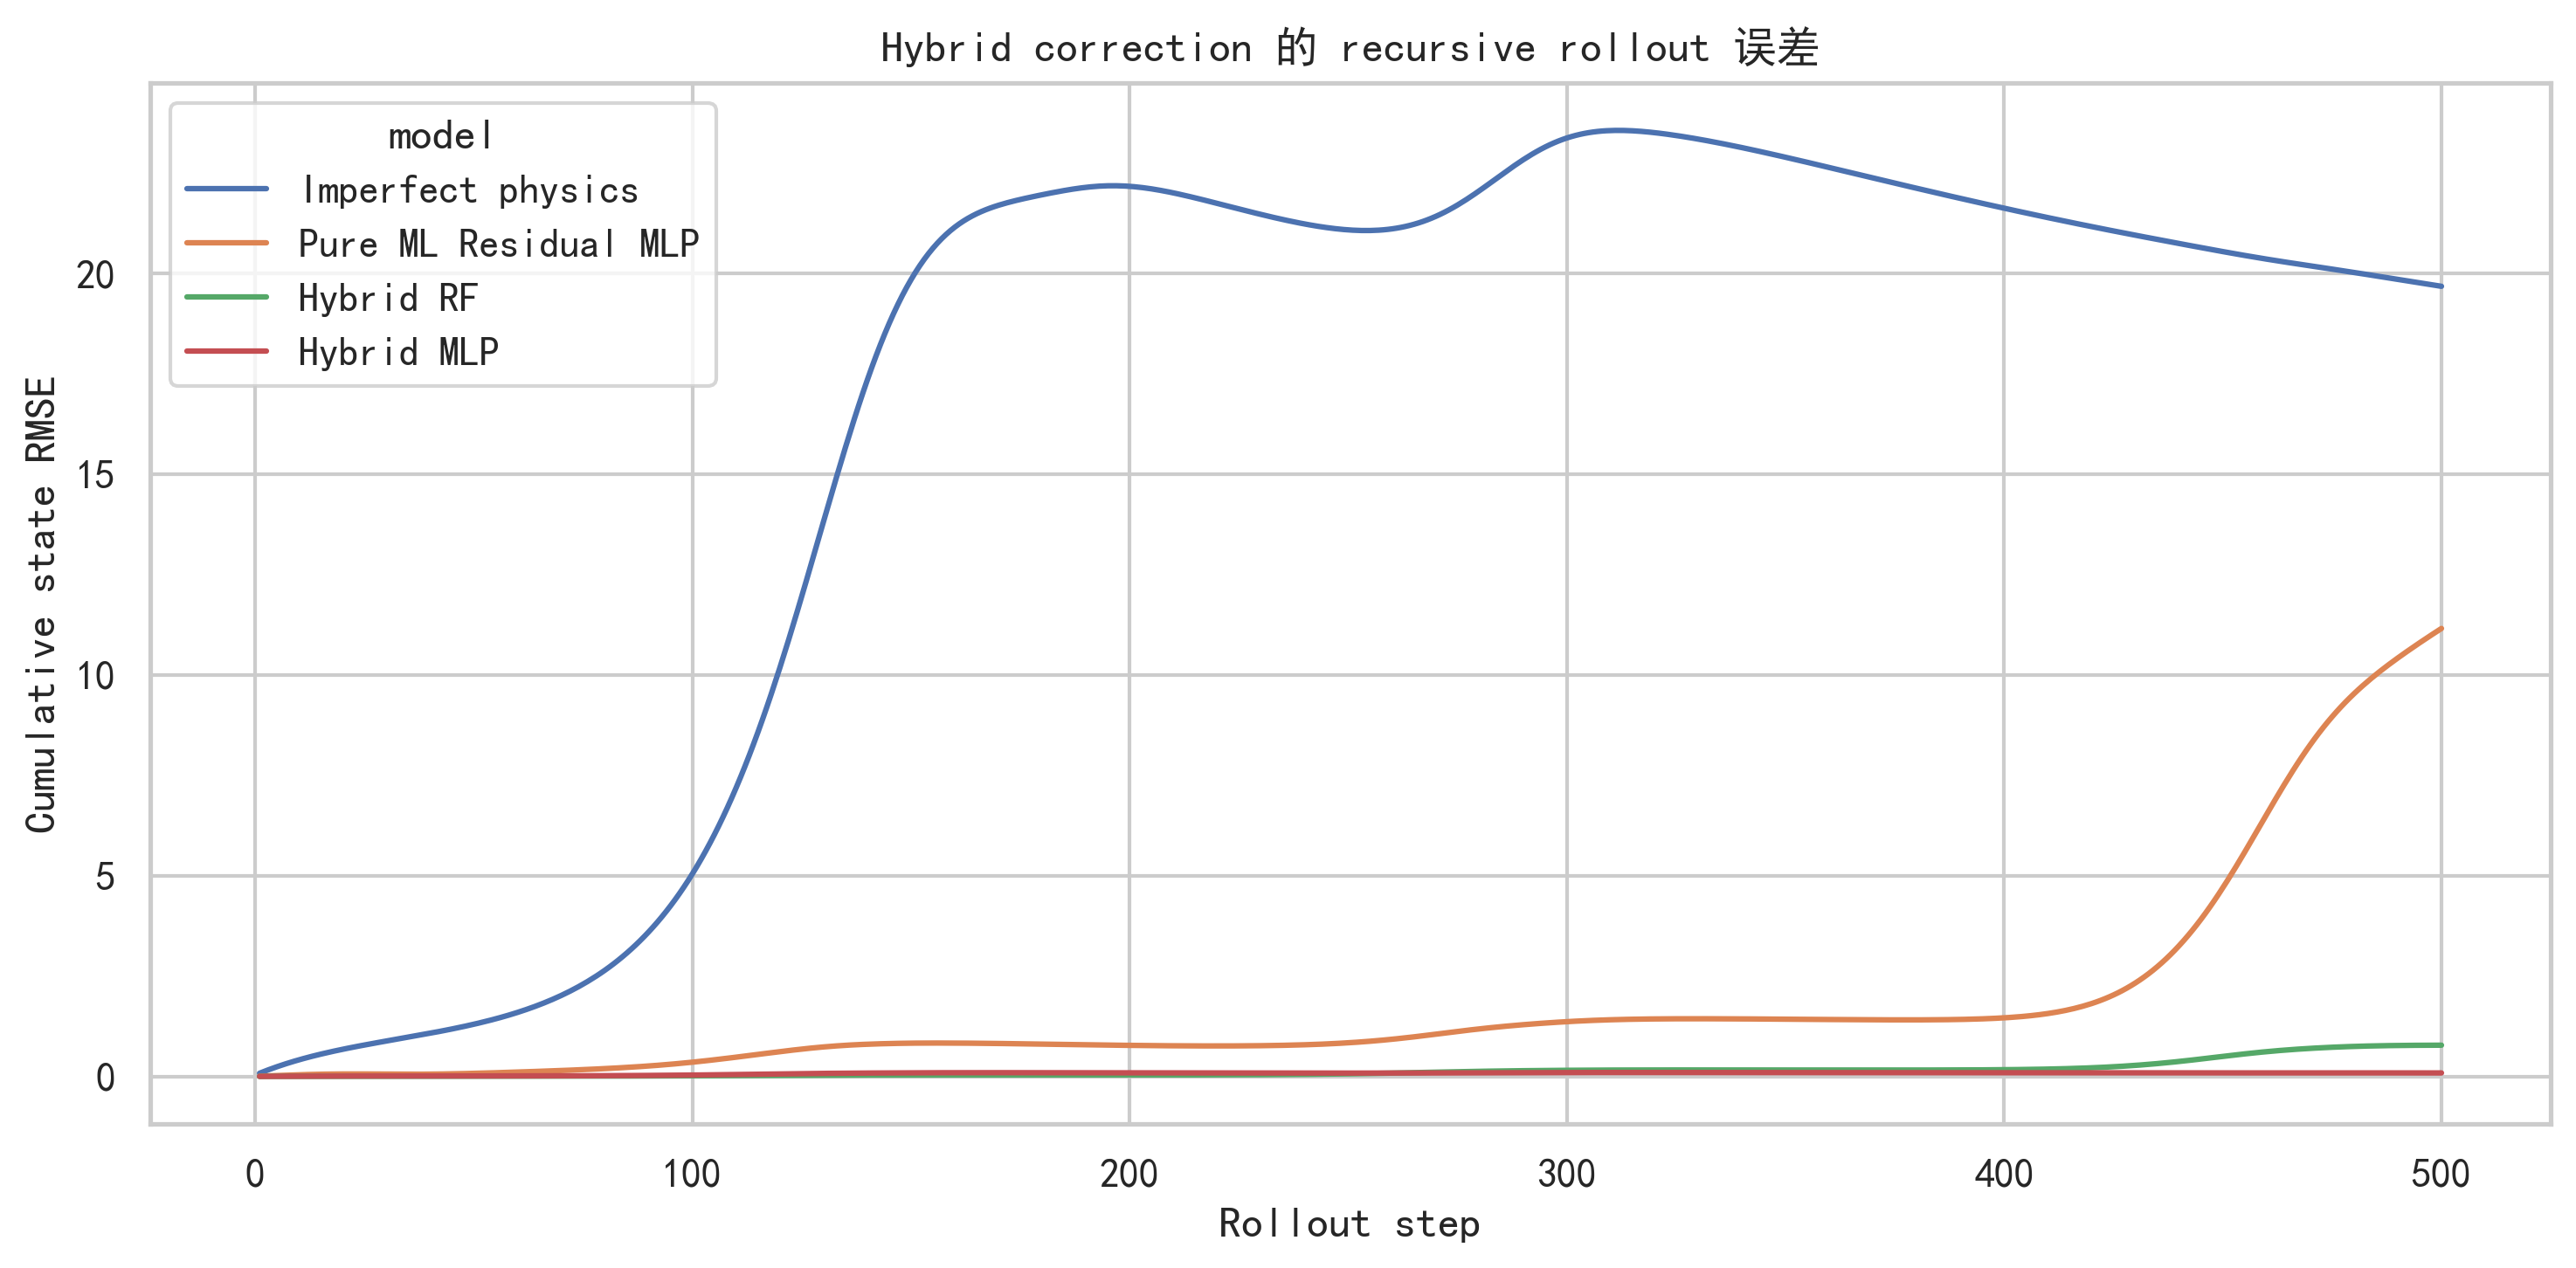
\includegraphics[width=0.88\textwidth]{figures/hybrid_rollout_error.png}
\caption{Hybrid correction 在递归多步预测中的累计状态 RMSE}
\label{fig:hybrid_rollout_error}
\end{figure}

\begin{figure}[H]
\centering
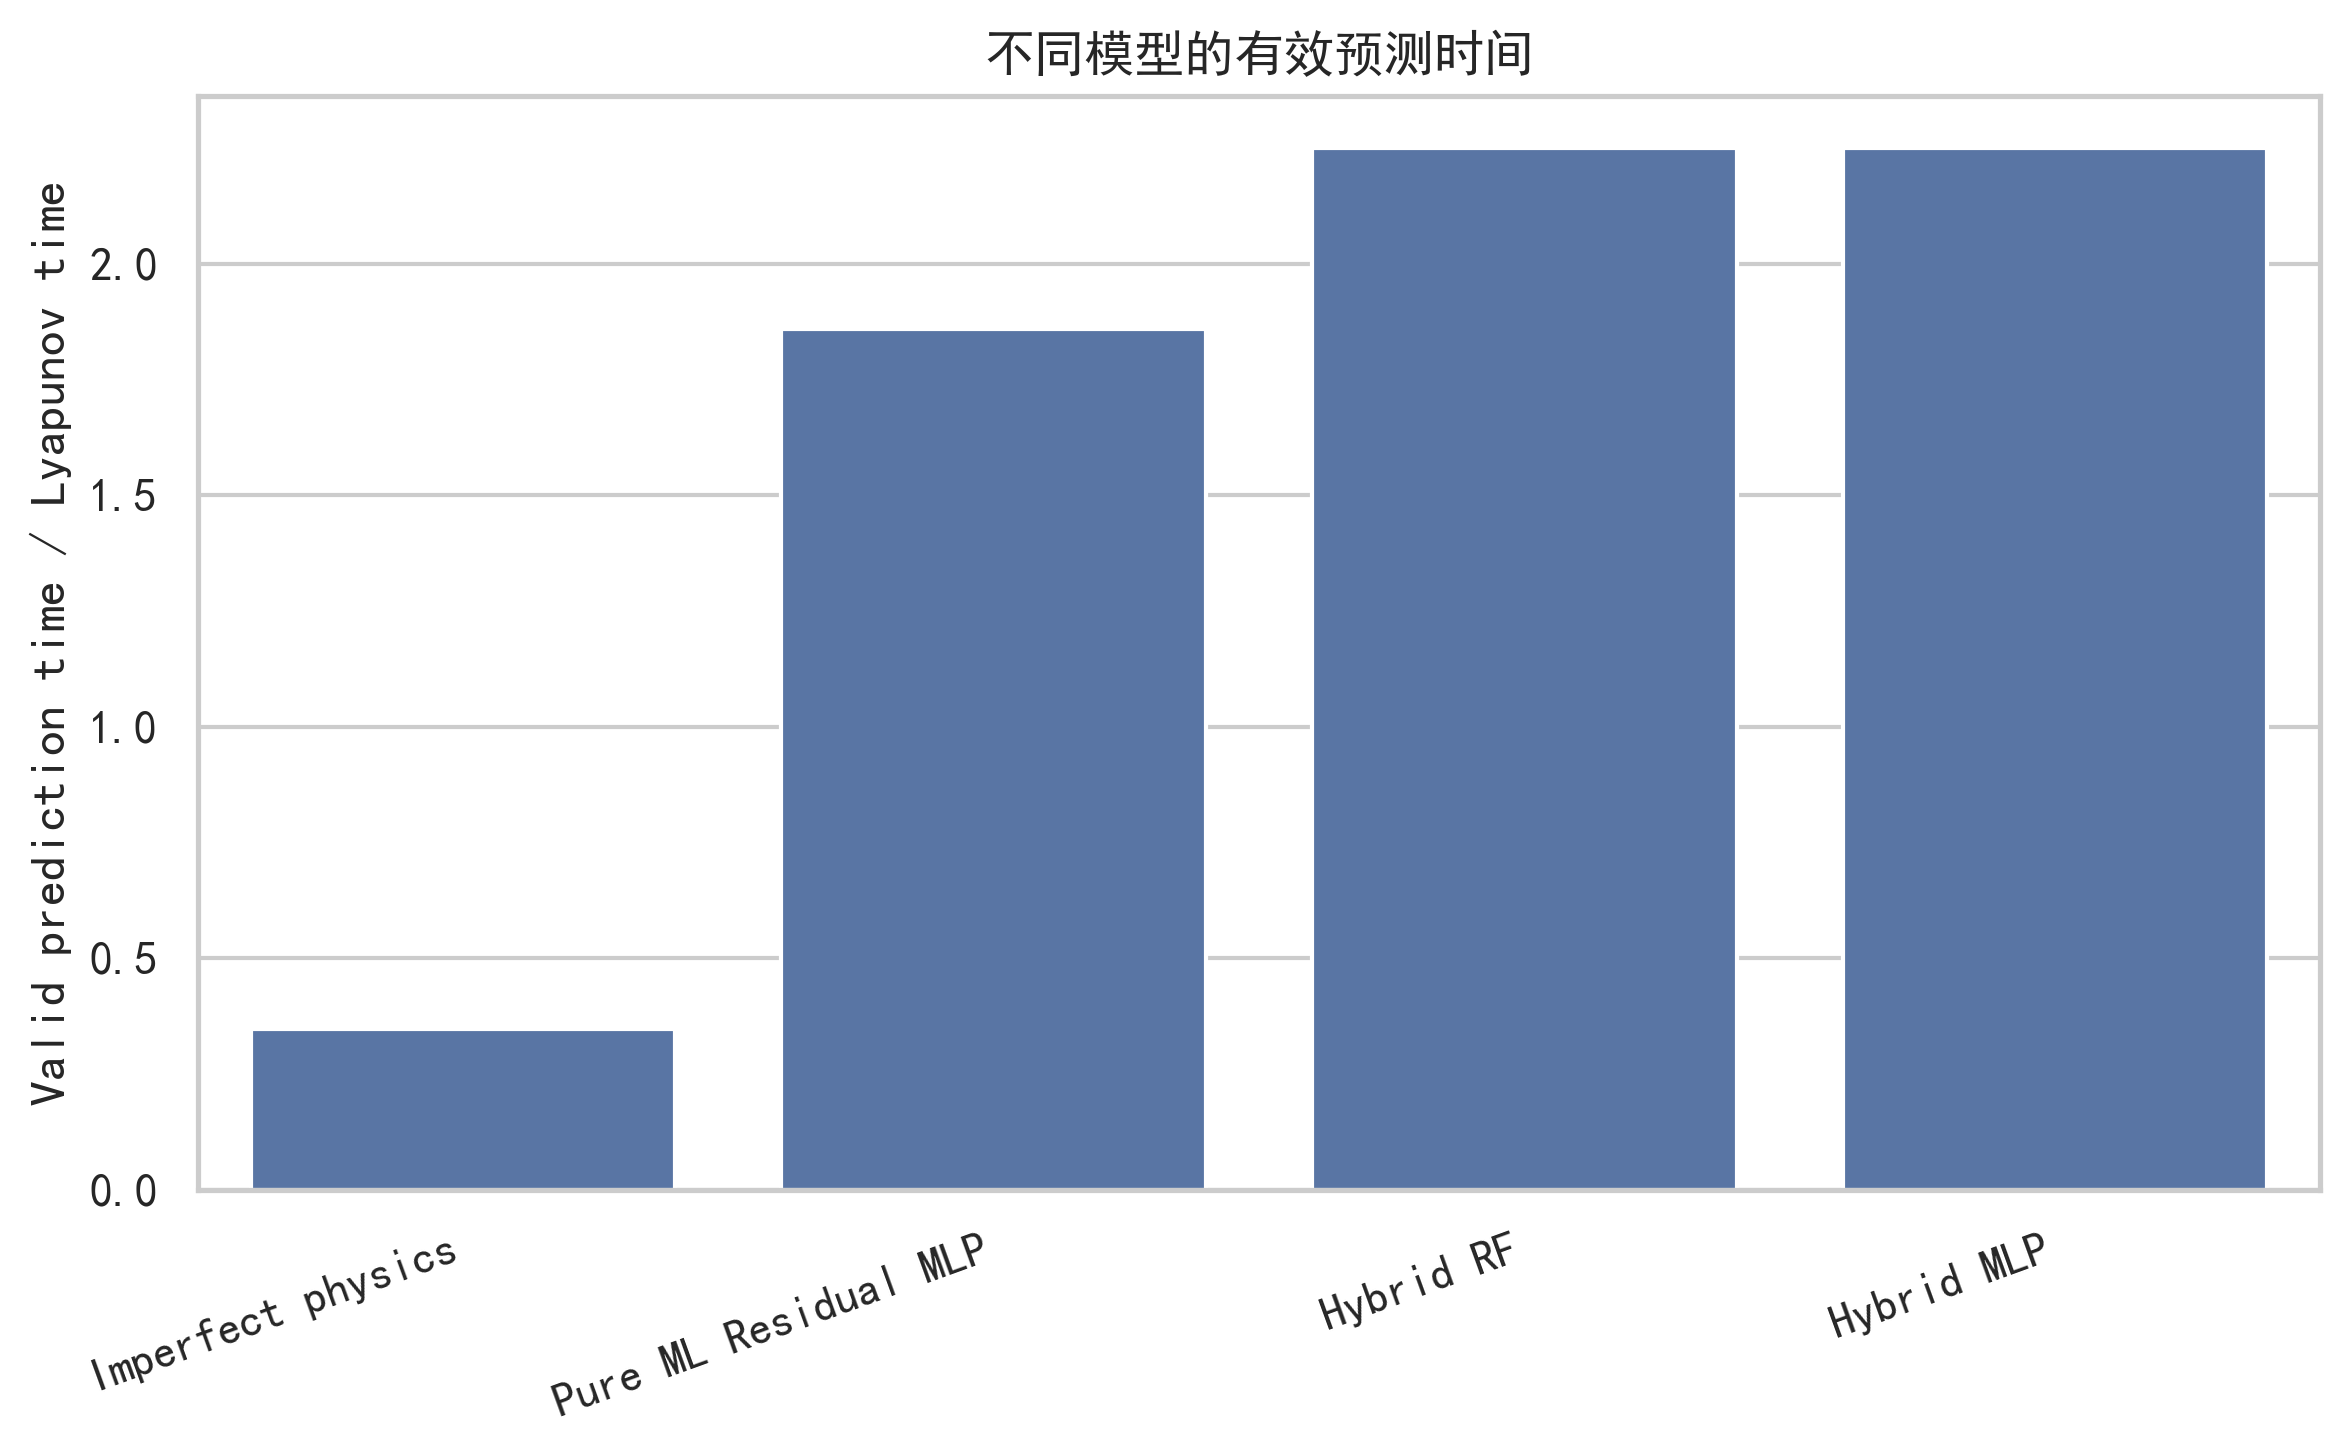
\includegraphics[width=0.82\textwidth]{figures/valid_prediction_time.png}
\caption{不同模型的有效预测时间（以 Lyapunov time 归一化）}
\label{fig:valid_prediction_time}
\end{figure}

最后，图 \ref{fig:long_term_distribution} 比较了真实轨迹与各模型 rollout 轨迹的长期分布。Hybrid MLP 的均值、标准差和分布形状与真实轨迹最接近，说明混合修正不仅改善逐点预测，也有助于保持吸引子的统计结构。

\begin{figure}[H]
\centering
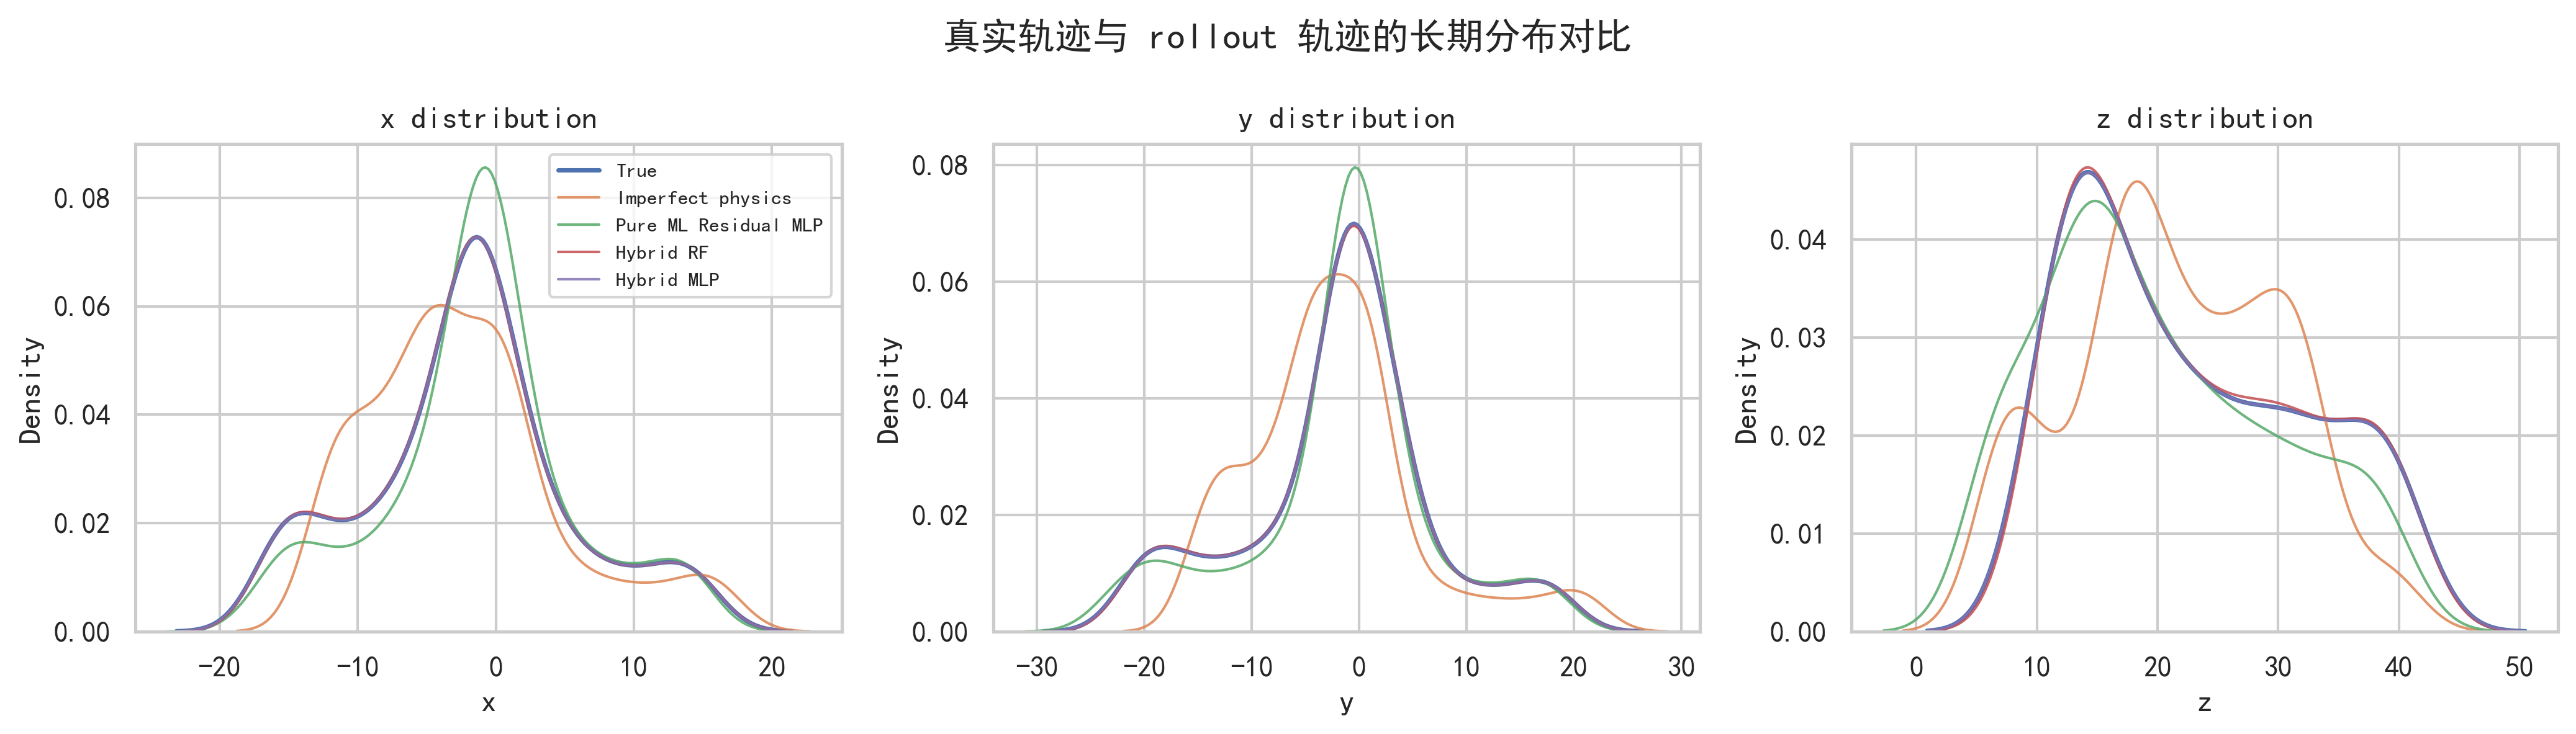
\includegraphics[width=0.95\textwidth]{figures/long_term_distribution_comparison.png}
\caption{真实轨迹与不同 rollout 轨迹的长期分布对比}
\label{fig:long_term_distribution}
\end{figure}

\section{讨论}

\subsection{为什么短期预测容易}

Lorenz 方程虽然会产生混沌轨迹，但系统本身仍由连续微分方程控制。在足够短的时间尺度内，状态不会发生任意跳变，当前状态与短期未来状态之间存在平滑的局部映射。因此，Random Forest、MLP 和 Residual MLP 在小预测步长下取得较低状态 RMSE 是合理的；这说明机器学习模型能够拟合局部状态转移，而不是说明长期轨迹已经变得容易预测。

\subsection{为什么长期预测困难}

当预测步长增大时，模型需要跨越更长时间的非线性演化，局部近似误差会被系统动力学放大。递归多步预测进一步加剧了这一问题：模型在每一步都使用自己的预测作为下一步输入，早期误差会改变后续输入分布，并持续影响之后的预测。不同初始条件实验也说明，模型的泛化质量依赖训练轨迹覆盖范围；新轨迹虽然来自同一方程和参数，但在相空间中的覆盖区域不同，误差水平也会变化。

\subsection{模型结构改进的作用与局限}

Residual MLP 的优势来自任务形式本身。对连续动力系统而言，学习状态增量 $\Delta\mathbf{s}$ 比直接学习未来状态更接近数值积分思想；输出标准化则能避免某个状态分量因尺度较大而主导损失。实验中，更深的 ReLU Residual MLP 在 $k=10$ 和 $k=100$ 上表现最好，而 tanh Residual MLP 在 rollout 中更稳定，说明结构设计和激活函数都会影响可预测窗口。

ESN 提供了动力系统时间序列模型视角，但本文中的轻量 ESN 并未全面超过 Residual MLP。尤其在较长步长的直接预测中，ESN residual 出现明显失效。这表明 reservoir computing 的效果依赖 reservoir 规模、谱半径、泄漏率和 readout 正则化等设置，不能简单认为加入 ESN 就一定优于普通 MLP。

\subsection{为什么 Hybrid correction 更符合 AI4SCI}

纯机器学习模型从数据中直接学习 $\mathbf{s}_t\to\mathbf{s}_{t+1}$，在短期内可以取得很低误差，但它没有显式利用 Lorenz 方程的结构。相反，Hybrid correction 先让不完美物理模型承担主要演化，再让机器学习只学习物理模型和真实系统之间的残差。这种分工降低了机器学习部分需要拟合的复杂度，也更接近真实科学计算场景：研究者通常拥有近似物理模型，但参数、边界条件或未建模项可能存在偏差。

本实验中，不完美物理模型只把 $\rho$ 从 28 改为 26，已经会在递归推演中快速偏离真实轨迹；而 Hybrid RF 和 Hybrid MLP 学到的残差修正显著延长了有效预测时间。这说明机器学习并不一定要替代物理模型，更有价值的用法是作为物理模型的误差校正器。

\subsection{本文局限}

本文仍是一个课程项目规模的实验研究。训练数据主要来自固定参数和有限初始条件下的模拟轨迹；模型只比较了若干常见机器学习方法、轻量 ESN、手写 SINDy 和简单 hybrid residual correction；ESN 和 SINDy 阈值未进行系统调参；Hybrid 实验只测试了 $\rho=26$ 这一种参数偏差。因此，本文更适合作为“短期可学、结构可识别、混合修正有效但长期受限”的预测边界分析，而不是对所有混沌系统预测方法的完整评测。

\section{结论}

本文将 Lorenz 混沌系统机器学习预测项目从单一 $x(t+10\Delta t)$ 短期预测扩展为完整三维状态转移预测，并进一步加入 SINDy 稀疏动力学识别和物理-机器学习混合修正。通过预测步长敏感性、递归多步预测、初始条件泛化、有效预测时间和长期统计分布，本文分析了模型在混沌系统中的预测边界。

实验表明，在固定参数和有限训练轨迹分布下，非线性机器学习模型能够有效近似 Lorenz 系统的短期局部状态转移映射；Residual MLP 和输出标准化可以改善短期与中期预测表现；SINDy 能从数据中恢复接近真实 Lorenz 方程的稀疏结构；Hybrid correction 能显著修正参数有偏的物理模型，并在本文设置中将有效预测时间提升到至少 2.25 个 Lyapunov time。

因此，本文的核心结论不是“机器学习已经解决混沌系统预测问题”，而是：机器学习可以学习 Lorenz 系统的短期局部动力学映射，稀疏识别可以揭示动力学方程结构，物理-机器学习混合修正可以扩大可预测窗口；但长期精确逐点预测仍受到混沌系统初值敏感性、误差放大和训练分布覆盖范围的限制。

未来工作可以进一步引入噪声鲁棒性测试、跨参数泛化实验、不同物理模型缺陷类型、horizon-conditioned MLP，以及对 ESN 的 reservoir 规模、谱半径、泄漏率和正则化系数进行系统调参。

\begin{thebibliography}{99}

\bibitem{lorenz1963}
Lorenz, E. N. (1963).
Deterministic nonperiodic flow.
\textit{Journal of the Atmospheric Sciences}, 20(2), 130--141.

\bibitem{pedregosa2011}
Pedregosa, F., Varoquaux, G., Gramfort, A., Michel, V., Thirion, B., Grisel, O., Blondel, M., Prettenhofer, M., Weiss, R., Dubourg, V., Vanderplas, J., Passos, A., Cournapeau, D., Brucher, M., Perrot, M., \& Duchesnay, E. (2011).
Scikit-learn: Machine learning in Python.
\textit{Journal of Machine Learning Research}, 12, 2825--2830.

\bibitem{virtanen2020}
Virtanen, P., Gommers, R., Oliphant, M., Haberland, M., Reddy, T., Cournapeau, D., Peterson, P., Weckesser, W., Bright, J., van der Walt, S., Brett, M., Wilson, J., Millman, K., Mayorov, N., Nelson, A., Jones, E., Kern, R., Larson, E., Carey, C., Polat, I., Feng, Y., Moore, E., VanderPlas, J., Laxalde, D., Perktold, J., Cimrman, R., Henriksen, I., Quintero, E., Harris, C., Archibald, A., Ribeiro, A., Pedregosa, F., \& van Mulbregt, P. (2020).
SciPy 1.0: Fundamental algorithms for scientific computing in Python.
\textit{Nature Methods}, 17, 261--272.

\bibitem{strogatz2015}
Strogatz, S. H. (2015).
\textit{Nonlinear Dynamics and Chaos: With Applications to Physics, Biology, Chemistry, and Engineering}.
Westview Press.

\bibitem{lukosevicius2009}
Luko\v{s}evi\v{c}ius, M., \& Jaeger, H. (2009).
Reservoir computing approaches to recurrent neural network training.
\textit{Computer Science Review}, 3(3), 127--149.

\end{thebibliography}

\appendix

\section{LLM 辅助说明}

本项目使用 LLM 辅助完成选题讨论、实验结构设计、Notebook 代码组织、结果解释和报告语言整理。所有实验结果均以实际运行的 Notebook、CSV 输出和图表文件为准；Lorenz 方程、数据切分、标准化流程、rollout 是否使用真实未来状态等关键环节均经过人工检查。

代表性提示词包括：

\begin{enumerate}
    \item “选择 Lorenz 混沌系统作为项目题目，并设计机器学习建模路线。”
    \item “请加入标准化、回归模型和 RMSE/MAE/$R^2$ 评价指标。”
    \item “请评估当前项目的研究深度，并提出更有说服力的实验增强方案。”
    \item “把项目增强为预测步长、三维状态预测、递归多步预测和跨初始条件泛化分析。”
    \item “比较 Direct MLP、Residual MLP、输出标准化、激活函数和 Echo State Network。”
\end{enumerate}

\end{document}
